\documentclass[12pt,a4paper,oneside]{book}
\usepackage[utf8]{vietnam}
\usepackage{amsmath, amsthm, amssymb,latexsym,amscd,amsfonts,enumerate,titlesec,titletoc}
\usepackage[top=3.0cm, bottom=3.0cm, left=3.5cm, right=2.0cm]{geometry}
% căn lề theo quy chuẩn KLTN
\usepackage{float}
\usepackage{color, fancyhdr, graphicx, wrapfig}
\usepackage[unicode]{hyperref}
\usepackage{indentfirst}
\usepackage{graphicx}
\usepackage{tikz}
\usepackage{array}
\usepackage{gensymb}
\usetikzlibrary{calc}
\usepackage[utf8]{inputenc}
\usepackage{pgfplots}
\pgfplotsset{compat=1.18} % Sử dụng phiên bản tương thích mới nhất
\usetikzlibrary{arrows.meta} % Để có thể tùy chỉnh đầu mũi tên tốt hơn nếu cần
\pgfplotsset{
    colormap={customviolet}{
        rgb255=(128,0,128) % Violet
        rgb255=(200,100,200) % Lighter violet
        rgb255=(255,150,200) % Pinkish
    }
}

%\newtheorem{example}{Ví dụ}[section]
\def\chaptertitlename{\fontsize{14pt}{14pt}\selectfont{CHƯƠNG}}
\titleformat{\chapter}[display]
{\vspace{-2cm}\normalfont\Large\filcenter\bfseries}
{{{\chaptertitlename\,}\thechapter}} {0pc}{{}\MakeUppercase}
\theoremstyle{theorem}
\newtheorem{theorem}{Định lý}[section]
\theoremstyle{definition}
\newtheorem{theorem2}{Định nghĩa}[section]
\newtheorem{dn}[theorem2]{Định nghĩa}
\newtheorem{nx}[theorem2]{Nhận xét}
\newtheorem{vd}[theorem2]{Ví dụ}
\newtheorem{md}[theorem2]{Mệnh đề}
\newtheorem{tc}[theorem2]{Tính chất}
\newtheorem{bd}[theorem2]{Bổ đề} 
\newtheorem{dl}[theorem2]{Định lí}
\newtheorem{bt}[theorem2]{Bài toán}
\newtheorem{hq}[theorem2]{Hệ quả}

%\newtheorem{example}{Ví dụ}[section]
%\newtheorem{proposition}{Mệnh đề}[section]
%\newtheorem{definition}[proposition]{Định nghĩa}
%\newtheorem{remark}[proposition]{Nhận xét}
%\newtheorem{theorem}[proposition]{Định lý}
%\newtheorem{example}[proposition]{Ví dụ}
%\newtheorem{corollary}[proposition]{Hệ quả}
%\newtheorem{lemma}[proposition]{Bổ đề}
\newtheorem{Theorem}{Theorem}[section]
\newtheorem{Proposition}[Theorem]{Proposition}
\newtheorem{Remark}[Theorem]{Remark}
\newtheorem{Lemma}[Theorem]{Lemma}
\newtheorem{Corollary}[Theorem]{Corollary}
\newtheorem{Definition}[Theorem]{Definition}
\newtheorem{Example}[Theorem]{Example}
\newcommand{\br}[1]{\left(#1\right)} %ngoặc tròn
\newcommand{\brb}[1]{\left\{#1\right\}} %ngoặc nhọn, tập hợp
\newcommand{\brc}[1]{\left[#1\right]} %ngoặc vuông
\newcommand{\bao}[1]{\left<#1\right>} 
\newcommand{\tri}[1]{\left|#1\right|}
\newcommand{\flo}[1]{ \left \lfloor #1 \right \rfloor}
\newtheorem*{case1}{Trường hợp 1}
\newtheorem*{case2}{Trường hợp 2}
\newtheorem*{case3}{Trường hợp 3}
\newcommand{\aut}[1]{\mbox{Aut}\br{#1}}
\newcommand{\gal}[1]{\mbox{Gal}\br{#1}}
\newcommand{\Q}{\mathbb{Q}}
\newcommand{\Z}{\mathbb{Z}}



\renewcommand{\theequation}{\thesection.\arabic{equation}}
\normalsize
\pagestyle{fancy}
\makeatletter
\renewcommand{\ps@plain}{
	\renewcommand{\@oddhead}{\textrm{\centerline{\thepage}}}
	\renewcommand{\@evenhead}{\@oddhead}
	\renewcommand{\@oddfoot}{}
	\renewcommand{\@evenfoot}{\@oddfoot}}
\pagestyle{plain}

%%%%%%%%%%%%%%%%%
\begin{document}
	\fontsize{13pt}{18pt}\selectfont % Lệnh thay đổi cỡ chữ thành cỡ 14, cỡ dòng 18 (theo quy chuẩn của Khóa Luận TN).
	\setlength{\baselineskip}{26truept}
	%\fontsize{13pt}{14pt}\selectfont
	\pagenumbering{arabic}
	%\pagenumbering{roman}
	%\frontmatter
	\pagestyle{empty}
	\begin{titlepage}
		
\begin{tikzpicture}[remember picture,overlay,inner sep=0,outer sep=0]
			\draw[black,line width=3pt] ([xshift=-1.5cm,yshift=-2cm]current page.north east) coordinate (A)--([xshift=2.85cm,yshift=-2cm]current page.north west) coordinate(B)--([xshift=2.85cm,yshift=2cm]current page.south west) coordinate (C)--([xshift=-1.25cm,yshift=2cm]current page.south east) coordinate(D)--cycle;
			
			\draw[black,line width=1pt] ([xshift=-1.7cm,yshift=-2.2cm]current page.north east) coordinate (A)--([xshift=3.05cm,yshift=-2.2cm]current page.north west) coordinate(B)--([xshift=3.05cm,yshift=2.2cm]current page.south west) coordinate (C)--([xshift=-1.45cm,yshift=2.2cm]current page.south east) coordinate(D)--cycle;
			
		\end{tikzpicture}
		\begin{center}
			\vspace{-1cm}\textbf{TRƯỜNG ĐẠI HỌC SƯ PHẠM, ĐẠI HỌC HUẾ}
			
			\vspace{7pt}
			\bf\underline{KHOA TOÁN HỌC}
		\end{center}
		\vspace{12pt}
		\begin{center}
			
			\vspace{1cm}
			\fontsize{17pt}{16pt}\selectfont 
			\textbf{HỌC PHẦN} 
			
			\vspace{6pt}
			\textbf{TÍCH HỢP CÔNG NGHỆ THÔNG TIN}\\
            \textbf{TRONG DẠY HỌC TOÁN}
		\end{center}

    
\begin{figure}[h]
    \centering
    \includegraphics[width=0.4\textwidth]{z7914774679386_4a58eb7c2cf50507f286bbe4918f13bf.jpg}
    \label{fig:enter-label}
\end{figure}
		\vspace{1.5cm}
		\begin{center}
			\fontsize{18pt}{17pt}\selectfont 
			\centerline 
            {\bf\fontsize{15pt}{28}\selectfont DỰ ÁN: ỨNG DỤNG CỦA HỆ PHƯƠNG TRÌNH ĐẠI SỐ}  

                \centerline {\bf\fontsize{15pt}{28}\selectfont TRONG GIẢI CÁC BÀI TOÁN THỰC TẾ}

 		\end{center}			
		\vspace{1cm}
		\begin{tabular}{cc}{\fontsize{13pt}{16}\selectfont   Giảng viên hướng dẫn}&\hspace{3.2cm}{\fontsize{13pt}{16}\selectfont Sinh viên thực hiện}\\
  {\bf\fontsize{12pt}{16}\selectfont NGUYỄN ĐĂNG MINH PHÚC}&\hspace{3.2cm}{\bf\fontsize{12pt}{16}\selectfont HOÀNG NGỌC HÙNG}\\ 
      &\hspace{3.2cm}{\bf\fontsize{13pt}{16}\selectfont MSSV: 23S1010011}
		\end{tabular}
		\vfill
		\centerline{\bf Huế, tháng 9 năm 2026}
\end{titlepage}
\newpage
\newpage
\markboth{{\it Mục lục}}{{\it Mục lục}}
%\addcontentsline{toc}{section}{{\bf Mục lục\rm }}
%\cleardoublepage

%{\protect\thispagestyle{empty}}
%%%%%%%%%%%%%%
%\include{Loicamdoan}
%\pagenumbering{arabic}
% \pagestyle{headings}
\newpage
\newpage

\def\@chapter[#1]#2{\ifnum \c@secnumdepth >\m@ne
                       \if@mainmatter
                         \refstepcounter{chapter}%
                         \typeout{\@chapapp\space\thechapter.}%
                         \addcontentsline{toc}{chapter}%
                              {\bf  Chương \protect\numberline{\thechapter. } #1}%
                       \else
                         \addcontentsline{toc}{chapter}{ #1}%
                       \fi
                    \else
                      \addcontentsline{toc}{chapter}{ #1}%
                    \fi
                    \chaptermark{#1}%
                    \addtocontents{lof}{\protect\addvspace{10\p@}}%
                    \addtocontents{lot}{\protect\addvspace{10\p@}}%
                    \if@twocolumn
                      \@topnewpage[\@makechapterhead{#2}]%
                    \else
                      \@makechapterhead{#2}%
                      \@afterheading
                    \fi}
%\setcounter{page}{3}
%%%%%%%%%%%%%%%%%%%%%%%
%\pagenumbering{roman}
\markboth{{\it Mục lục}}{{\it Mục lục}}
\tableofcontents
\pagestyle{plain}
\chapter*{LỜI CẢM ƠN}
\fontsize{13pt}{22pt} \selectfont
Để hoàn thành dự án \textit{“Ứng dụng của hệ phương trình đại số trong giải các bài toán thực tế”}, tôi đã nhận được rất nhiều sự giúp đỡ, hướng dẫn và động viên trong suốt quá trình học tập và nghiên cứu.

Trước tiên, tôi xin gửi lời tri ân chân thành và sâu sắc đến Giảng viên TS. Nguyễn Đăng Minh Phúc — người đã trực tiếp hướng dẫn, tận tình chỉ bảo và luôn dành nhiều thời gian hỗ trợ tôi trong quá trình thực hiện dự án. Những kiến thức, nhận xét và góp ý của giảng viên đã giúp tôi có thêm định hướng để hoàn thiện dự án này.

Tôi cũng xin chân thành cảm ơn Ban Chủ nhiệm khoa Toán cùng quý thầy cô trong khoa đã tạo điều kiện thuận lợi về học tập và nghiên cứu. Đồng thời, tôi xin cảm ơn các bạn sinh viên đã nhiệt tình chia sẻ tài liệu, đóng góp ý kiến và động viên tôi trong suốt thời gian thực hiện đề tài.

Do kiến thức và kinh nghiệm nghiên cứu còn hạn chế, dự án chắc chắn vẫn còn những thiếu sót nhất định. Tôi rất mong nhận được những ý kiến đóng góp quý báu từ quý thầy cô và các bạn để bài viết được hoàn thiện hơn.

Xin chân thành cảm ơn!

\begin{flushright}
Huế, tháng 9 năm 2026\\[0.3cm]
\textbf{Sinh viên thực hiện}
\end{flushright}

\addcontentsline{toc}{chapter}{LỜI CẢM ƠN}

	%\chapter*{\huge MỞ ĐẦU}
	%\addcontentsline{toc}{chapter}{MỞ ĐẦU}
    \chapter*{MỞ ĐẦU}
    \addcontentsline{toc}{chapter}{MỞ ĐẦU}
Trong toán học, hệ phương trình đại số là một nội dung quan trọng và được sử dụng khá phổ biến. Không chỉ xuất hiện trong các bài toán ở trường học, hệ phương trình còn có mặt trong nhiều lĩnh vực khác như vật lí, kinh tế, kĩ thuật hay công nghệ thông tin. Nhiều vấn đề trong thực tế có thể được giải quyết thông qua việc thiết lập và tìm nghiệm của hệ phương trình phù hợp.

Việc tìm hiểu các phương pháp giải hệ phương trình giúp người học nâng cao khả năng tư duy, phân tích và xử lí bài toán. Ngoài những phương pháp cơ bản thường gặp, còn có nhiều cách biến đổi linh hoạt giúp việc giải toán trở nên hiệu quả hơn. Qua đó, người học có thể rèn luyện được tư duy logic và khả năng vận dụng kiến thức vào thực tế.

Trong tiểu luận này, nội dung chủ yếu tập trung vào việc trình bày các kiến thức cơ bản về hệ phương trình đại số, giới thiệu một số phương pháp giải thường dùng và phân tích các dạng hệ phương trình quen thuộc. Đồng thời, bài viết cũng đề cập đến một vài ứng dụng đơn giản của hệ phương trình trong học tập và đời sống.

Đề tài chủ yếu nghiên cứu các hệ phương trình đại số hữu hạn với hai hoặc ba ẩn số. Những nội dung chuyên sâu như hệ phương trình vi phân hoặc các dạng hệ phức tạp khác sẽ không được trình bày chi tiết trong phạm vi tiểu luận này.

Nội dung của bài tiểu luận được trình bày thành ba chương chính như sau:

\textit{Chương 1. Tổng quan về hệ phương trình và hệ phương trình đại số}

Trình bày các khái niệm cơ bản liên quan đến hệ phương trình, đồng thời giới thiệu một số phương pháp giải thường gặp đối với các dạng hệ phương trình quen thuộc như phương pháp thế, phương pháp cộng đại số, phương pháp đặt ẩn phụ,...

\textit{Chương 2. Một số hệ phương trình đại số và phương pháp giải}

Tập trung phân loại các dạng hệ phương trình đại số thường gặp và trình bày các phương pháp giải phù hợp đối với từng dạng, từ hệ phương trình tuyến tính đến một số hệ phương trình phi tuyến cơ bản.

\textit{Chương 3. Ứng dụng của hệ phương trình đại số trong thực tiễn}

Trình bày một số ứng dụng của hệ phương trình đại số trong học tập và đời sống thực tế, đặc biệt là các bài toán liên quan đến hệ phương trình tuyến tính, qua đó minh họa vai trò và ý nghĩa của hệ phương trình trong thực tiễn.

%Phần 1%

    \chapter{TỔNG QUAN VỀ HỆ PHƯƠNG TRÌNH}
    \section{Định nghĩa}
    \begin{dn}
        Trong $\mathbb{R}^n$, cho $m$ phương trình
        \[
\begin{aligned}
f_1(x) &= g_1(x) \\
f_2(x) &= g_2(x) \\
&\vdots \\
f_m(x) &= g_m(x)
\end{aligned}
\]

Trong đó $f_i(x),g_i(x),i=1;2;...;m$ là các hàm $n$ biến với $x=(x_1;x_2;...;x_n)$ được gọi là \textit{ẩn}.

Giả sử $m$ phương trình trên lần lượt có các tập xác định là $D_i,\, i=1;2;...;m$.

Khi đó $m$ phương trình trên lập thành một hệ các phương trình được gọi là \textit{hệ $m$ phương trình $n$ ẩn} hay \textit{hệ $m$ phương trình}. Kí hiệu là
\[
\left\{
\begin{aligned}
f_1(x) &= g_1(x) \\
f_2(x) &= g_2(x) \\
&\vdots \\
f_m(x) &= g_m(x)
\end{aligned}
\right.
\tag{*}
\]

Hệ $(*)$ có tập xác định là $D=\bigcap_{i=1}^{m}{D_i}$.
    \end{dn}
    \begin{dn}
        Hệ $m$ phương trình $(*)$ được gọi là \textit{hệ m phương trình đại số} nếu $m$ phương trình đều là các phương trình đại số (phương trình chỉ chứa ẩn và các phép toán đại số như cộng, trừ, nhân, chia, lũy thừa với số mũ hữu tỉ hoặc nguyên).
    \end{dn}
 \newpage
    Trong phần sau của bài tiểu luận này (do không có sự nhẫm lẫn) khi viết \textit{hệ phương trình} nếu không giải thích gì thêm sẽ được hiểu là \textit{hệ phương trình đại số}.
  
    \begin{vd} Ta có thể lấy vài ví dụ:
    \begin{enumerate}
    
      \item \[\left\{
\begin{aligned}
x+3 &= y-2z+5 \\
y &= 2x-1 \\
7z-1 &= 3x^2+4y^2
\end{aligned}
\right.\]

là một hệ 3 phương trình đại số với 3 ẩn là $x,y,z$.
    
    \item \[\left\{
\begin{aligned}
e^{3x+2} &= 4y+5 \\
ln(2y-9)&= 6x-1 \\
5z^2-3 &=4t^2+6y^2
\end{aligned}
\right.\]

    là một hệ 3 phương trình với 4 ẩn là $x,y,z,t$. Hệ phương trình này không phải là hệ phương trình đại số vì có xuất hiện hàm $e^{3x+2}$ và $ln(2y-9)$ không phải hàm đại số. 
 \end{enumerate}
    \end{vd}
    
    \begin{dn}
        Cho hệ $m$ phương trình $n$ ẩn có tập xác định $D$
\begin{equation}
\left\{
\begin{aligned}
f_1(x) &= g_1(x) \\
f_2(x) &= g_2(x) \\
&\vdots \\
f_m(x) &= g_m(x)
\end{aligned}
\right.
\end{equation}

Mỗi giá trị $a=(a_1;a_2;...;a_n) \in D$ được gọi là \textit{nghiệm của hệ phương trình} $(1.1.1)$ nếu khi thay $x=(x_1;x_2;...;x_n)$ bằng $a=(a_1;a_2;...;a_n)$  vào tất cả phương trình trong $(1.1.1)$ đều được đẳng thức đúng.

Ta kí hiệu tập tất cả các nghiệm của $(1.1.1)$ là $S$ khi đó $S=\bigcap_{i=1}^m{S_i}$ với $S_i$ là tập nghiệm của phương trình thứ $i$.

Nếu $S=\emptyset$ thì ta nói hệ phương trình $(1.1.1)$ vô nghiệm.
    \end{dn}
    \begin{vd}
        \[
\left\{
\begin{aligned}
&x+y+z &= 6 \\
&x-y+z&= 2 \\
&x+y-z &= 4
\end{aligned}
\right.
\]
Ta có thể thấy $a=(3;2;1)$ là một nghiệm của hệ phương trình trên do khi thay  $(x;y;z)=(3;2;1)$ vào cả $3$ phương trình của hệ ta đều được đẳng thức đúng.
    \end{vd}
 \section{Các phương pháp tổng quát giải hệ phương trình đại số}   
        \subsection{Phương pháp thế}
       \subsubsection{Phương pháp giải:} Với hệ gồm $ n$ phương trình $n$ ẩn: 
       \begin{enumerate}
       
             \item Chọn một phương trình của hệ rút một ẩn theo các ẩn còn lại.
             \item Thế ẩn vừa tìm được vào các phương trình còn lại. Ta được hệ gồm $n-1$ phương trình với $n-1$ ẩn.
             \item Lặp lại bước đầu tiên cho hệ mới cho đến khi còn duy nhất một phương trình với một ẩn hoặc xuất hiện một phương trình trong hệ phương trình mới là phương trình một ẩn.
             \item Giải phương trình một ẩn, rồi thế ngược lại vào các phương trình vừa rút để tìm các ẩn còn lại.
       \end{enumerate}
       
      
        \begin{vd}
        Tìm tập nghiệm của hệ phương trình sau bằng phương pháp thế:
    \[
\left\{
\begin{aligned}
&3x+2y-z &= 1 \\
&2x+y&= 2 \\
&2x+y+z &= 5
\end{aligned}
\right.
\]
       \end{vd}
         \textbf{\textit{Lời giải.}}
         
         Rút $y$ ở phương trình thứ hai ta được $y=2-2x$, thay vào hai phương trình còn lại ta được hệ phương trình mới là 
 
\[
\begin{cases}
\begin{aligned}
&3x+2(2-2x)-z &= 1 \\
&2x+(2-2x)+z &= 5
\end{aligned}
\end{cases}
\Leftrightarrow
\begin{cases}
\begin{aligned}
&-x-z &= -3 \\
&2 +z&=5
\end{aligned}
\end{cases}
\]

Rút $z=5-2=3$ từ phương trình thứ hai. Ta thế $z=3$ vào phương trình còn lại suy ra được $x=-3+3=0$

Để ý ta đã rút $y=2-2x$ nên sau khi đã tìm được $x=2$ ta chỉ cần thế ngược lại để tìm y. Do đó $y=2-2.2=-2$

Vậy hệ phương trình trên có nghiệm là $(2;-2;3)$.

\begin{vd}
        Tìm tập nghiệm của hệ phương trình sau bằng phương pháp thế:
    \[
\left\{
\begin{aligned}
&6x+4y-z &= 0 \\
&2x+y&= 1 \\
&4x+2y &= 2
\end{aligned}
\right.
\]
       \end{vd}
     \textbf{\textit{Lời giải.}}\\
Ta có: \[
\begin{cases}
\begin{aligned}
&6x+4y-z &= 0 \\
&2x+y&= 1 \\
&4x+2y &= 2
\end{aligned}
\end{cases}
\Leftrightarrow
\begin{cases}
\begin{aligned}
&3(2x+y)+y-z &= 0 \\
&2x+y&= 1 \\
&2(2x+y) &= 2
\end{aligned}
\end{cases} \]

Thay phương trình thứ hai $2x+y= 1$ vào hai phương trình còn lại ta được hệ mới là

\[
\left\{
\begin{aligned}
&y-z +3&= 0 \\
&2 &= 2
\end{aligned}
\right.
\] 

Phương trình duy nhất còn lại sau khi thế là $y-z+3=0$ phương trình này vô số nghiệm, với $y=z-3$ phụ thuộc vào ẩn $z$.

Rút $x$ từ phương trình $2x+y=1$ ta được $x=\frac{1}{2}(1-y)=\frac{1}{2}(1-z+3)= \frac{1}{2}(4-z)$.

Vậy hệ phương trình trên có vô số nghiệm dạng $\{(\frac{1}{2}(4-z);z-3;z)| \hspace{0.2cm} z \in \mathbb{R}\}$.
\begin{nx}

    \begin{itemize}
        \item Số nghiệm của hệ phương trình ban đầu phụ thuộc vào số nghiệm của phương trình cuối cùng sau khi rút hết các ẩn của phương trình khác trong hệ.
        \item Có nhiều cách rút và thế tùy vào tình huống bài toán.
        \item Nếu các phương trình trong hệ có chứa một phần của các phương trình khác thì ta có thể thay các phương trình đó vào phương trình này. 
        
        Ví dụ như trong \textbf{Ví dụ 1.2.2} ta thấy phương trình đầu tiên có xuất hiện \textit{$2x+y$} trong \textit{$3(2x+y)+y-z=0$} và \textit{$2(2x+y)=2$} mà \textit{$2x+y=1$} nên ta thay vào hai phương trình còn lại và được hệ phương trình mới như trên bài giải.
    \end{itemize}
\end{nx}
        \subsection{Phương pháp cộng đại số}
        \subsubsection{Phương pháp giải:}
         Với hệ gồm $ n$ phương trình $n$ ẩn như sau:
           \[ \begin{cases}
        
\begin{aligned}
a_{11}x_1+a_{12}x_2+...+a_{1n}x_n &=a_1 \\
a_{21}x_1+a_{22}x_2+...+a_{2n}x_n &=a_2 \\
\dots \\
a_{n1}x_1+a_{n2}x_2+...+a_{nn}x_n &=a_n
\end{aligned}
           \end{cases}
\]

Trong đó $a_{ij} \in \mathbb{R}, \forall i, j \in \{1; 2;...;n\}$ là các hệ số, $x_1;...x_n$ là các ẩn.
       \begin{enumerate}
       
             \item Ta lần lượt nhân các số $b_i\neq0$ vào phương trình thứ $i$ sao cho khi lấy phương trình thứ nhất lần lượt cộng với phương trình thứ $i$ thì hệ số đi với ẩn $x_1$ là bằng 0.
             \item Giữ nguyên phương trình đầu tiên còn các phương trình thứ $i$ thì thay bằng phương trình mới chính là tổng của phương trình đầu tiên với phương trình đó.
             \item Lần lượt lặp lại thao tác này đối với hệ số của ẩn $x_2,x_3,...$ cho đến khi phương trình được giữ nguyên là phương trình một ẩn.
             \item Giải phương trình một ẩn để tìm ra nghiệm $x_i$ sau đó thế giá trị này vào các phương trình còn lại để giải ra nghiệm tổng quát của hệ phương trình.

             \begin{vd} Giải hệ phương trình sau:

\[
\left\{
\begin{aligned}
x_1+x_2+x_3+x_4 &= 2\\
x_1+x_2+2x_3+3x_4 &= 5\\
2x_1+3x_2+x_3+2x_4 &= 4\\
x_1+2x_2+3x_3+x_4 &= 3
\end{aligned}
\right.
\]

\textbf{Lời giải.}

Lấy phương trình thứ hai trừ phương trình thứ nhất, phương trình thứ ba trừ hai lần phương trình thứ nhất và phương trình thứ tư trừ phương trình thứ nhất, ta được hệ phương trình mới như sau:

\[
\left\{
\begin{aligned}
x_1+x_2+x_3+x_4 &= 2\\
x_3+2x_4 &= 3\\
x_2-x_3 &= 0\\
x_2+2x_3 &= 1
\end{aligned}
\right.
\]

Giữ nguyên phương trình thứ ba, phương trình thứ tư thay bằng hiệu của phương trình thứ tư và phương trình thứ ba, ta được:

\[
\left\{
\begin{aligned}
x_1+x_2+x_3+x_4 &= 2\\
x_3+2x_4 &= 3\\
x_2-x_3 &= 0\\
3x_3 &= 1
\end{aligned}
\right.
\]
Ta thấy phương trình thứ tư là phương trình một ẩn, giải phương trình này ta được:
\[
x_3=\frac13
\]
Thay \(x_3=\dfrac13\) vào phương trình thứ ba ta được:
\[
x_2=\frac13
\]
Thay \(x_3=\dfrac13\) vào phương trình thứ hai ta được:
\[
\frac13+2x_4=3
\]
\[
2x_4=\frac83
\]
\[
x_4=\frac43
\]
Thay tất cả các giá trị vừa tìm được vào phương trình thứ nhất ta được:
\[
x_1+\frac13+\frac13+\frac43=2
\]
\[
x_1+2=2
\]
\[
x_1=0
\]
Vậy nghiệm của hệ phương trình trên là:
\[
\boxed{\left(0,\frac13,\frac13,\frac43\right)}
\]
             
\begin{nx}
     \begin{itemize}
        \item Cũng giống như phương pháp thế số nghiệm của hệ phương trình ban đầu phụ thuộc vào số nghiệm của phương trình cuối cùng sau khi biến đổi hệ phương trình.
        \item Phương pháp này chỉ được sử dụng đối với những hệ phương trình dạng tuyến tính như đã được nêu ở phần phương pháp.
        \item Không nhất thiết là sẽ dùng phương trình đầu tiên làm mốc, ta có thể thay đổi cách chọn tùy vào hệ phương trình, để ý thấy hệ số "đẹp" để biến đổi tránh làm phức tạp bài toán.
        
    \end{itemize}
\end{nx}
             \end{vd}
       \end{enumerate}
       \subsection{Phương pháp biến đổi tương đương}
       \subsubsection{Phương pháp giải:}
       \begin{itemize}
           \item Phương pháp này đưa hệ phương trình thành hệ đơn giản hơn bằng cách biến đổi các phương trình trong hệ mà không thay đổi tập nghiệm của phương trình.
           \item Các phép biến đổi tương đương phổ biến: Thay đổi vị trí của các phương trình, nhân một (hay một số) phương trình với hệ số $a\neq0$ nào đó, phương pháp cộng đại số cũng là một trường hợp của phương pháp biến đổi tương đương,v.v.
           \item Ta có thể áp dụng nhiều phương pháp biến đổi tương đương cùng một lúc cho một hệ phương trình.
           Ví dụ: trong một hệ phương trình ta có thể lấy phương trình đầu tiên cộng với $k\neq0$ lần phương trình thứ hai chẳng hạn.
       \end{itemize}
       \begin{vd}
      Giải hệ phương trình sau bằng phương pháp biến đổi tương đương:
\[
\left\{
\begin{aligned}
x+y &= 5\\
2x-y &= 4
\end{aligned}
\right.
\]
\textbf{Lời giải.}
Giữ nguyên phương trình thứ nhất, cộng phương trình thứ nhất với phương trình thứ hai, ta được hệ phương trình mới:
\[
\left\{
\begin{aligned}
x+y &= 5\\
3x &= 9
\end{aligned}
\right.
\]
Ta thấy phương trình thứ hai là phương trình một ẩn, giải phương trình này ta được:
\[
x=3
\]
Thay \(x=3\) vào phương trình thứ nhất ta được:
\[
3+y=5
\]
\[
y=2
\]
Vậy nghiệm của hệ phương trình trên là:
\[
\boxed{(3,2)}
\]
\end{vd}
     \subsection{Phương pháp đặt ẩn phụ}
        \subsubsection{Phương pháp giải:}
        Đối với hệ phương trình $n$ ẩn phi tuyến tính phức tạp tuy nhiên có nhiều điểm chung tại các ẩn ở các phương trình trong hệ ta có thể giải quyết như sau:
        \begin{enumerate}
            \item Xem xét các điểm chung của các phương trình. Đặt các điểm chung đó với hệ ẩn mới.
            \item Thay hệ ẩn mới vào hệ và giải quyết bằng các phép biến đổi tương đương hoặc các phương pháp khác.
            \item Sau khi giải ra hệ ẩn mới thì ta lần lượt thay các giá trị vào hệ ẩn vừa tìm để giải ra được giá trị của ẩn ban đầu.
        \end{enumerate}
  
  \begin{vd}Giải hệ phương trình sau:

\[
\left\{
\begin{aligned}
x^2+y^2-2x-4y &= 1\\
x^2-4y^2-2x+16y &= -4
\end{aligned}
\right.
\]

\textbf{Ý tưởng.} 

Ta nhận thấy:
\[x^2-2x=(x-1)^2-1\]
và
\[y^2-4y=(y-2)^2-4
\]
Do đó phương trình thứ nhất có thể đưa về dạng chứa
\((x-1)^2\) và \((y-2)^2\).
Ở phương trình thứ hai ta cũng có:
\[x^2-2x=(x-1)^2-1
\]
và\[-4y^2+16y=-4[(y-2)^2-4]
\]
Khi ấy hệ phương trình đã cho tương đương với:
\[
\left\{
\begin{aligned}
(x-1)^2+(y-2)^2 &= 6\\
(x-1)^2-4(y-2)^2 &= -13
\end{aligned}
\right.
\]
Khi này ta có thể đặt:
\[u=(x-1)^2,\qquad v=(y-2)^2
\]
để đưa hệ đã cho về hệ phương trình tuyến tính.

\textbf{Lời giải.}
Đặt
\[
\left\{
\begin{aligned}
u&=(x-1)^2,\qquad u\ge0\\
v&=(y-2)^2,\qquad v\ge0
\end{aligned}
\right.
\]
Hệ phương trình đã cho tương đương với:
\[
\left\{
\begin{aligned}
u+v &= 6\\
u-4v &= -13
\end{aligned}
\right.
\]
Giải hệ trên ta được:
\[
\left\{
\begin{aligned}
u&=\frac{11}{5}\\
v&=\frac{19}{5}
\end{aligned}
\right.
\]
Do đó:
\[(x-1)^2=\frac{11}{5}
\]
suy ra
\[x=1\pm\sqrt{\frac{11}{5}}
\]
và
\[(y-2)^2=\frac{19}{5}
\]
suy ra
\[y=2\pm\sqrt{\frac{19}{5}}
\]
Vậy hệ phương trình đã cho có các nghiệm:
\[
\boxed{
\left(1\pm\sqrt{\frac{11}{5}},\,
2\pm\sqrt{\frac{19}{5}}\right)
}
\]
  \end{vd}

\textbf{Khi sử dụng phương pháp đặt ẩn phụ cần chú ý:}
\begin{itemize}
    \item Chọn ẩn phụ phù hợp để hệ mới đơn giản hơn hệ ban đầu;
    \item Đặt đầy đủ điều kiện cho ẩn phụ nếu cần;
    \item Sau khi giải hệ theo ẩn phụ phải quay lại tìm các ẩn ban đầu;
    \item Kiểm tra nghiệm thu được với điều kiện xác định của hệ.
\end{itemize}
\begin{nx}
\begin{itemize}
    \item Phương pháp này giúp đưa một hệ phương trình với các ẩn và hệ số phức tạp về phương trình đơn giản hơn.
    \item Phương pháp này tuy hữu ích cho các hệ phương trình phức tạp tuy nhiên nên để ý các dấu hiệu của các phương trình để chọn cách đặt phù hợp.
    \item Mỗi dạng hệ phương trình có nhiều cách đặt khác nhau tùy dụng ý của bài toán.
\end{itemize}    
\end{nx}

            \subsection{Phương pháp biểu diễn hình học}
        \subsubsection{Phương pháp giải:}
Đối với những hệ phương trình có các phương trình dạng hàm số (hoặc có thể đưa về hàm số), có thể miêu tả thông qua đồ thị của một đường đã biết (elip, đường tròn,v.v.), v.v.
\begin{enumerate}
    \item Đưa các phương trình về dạng hàm số, phương trình của các đường quen thuộc.
    \item Vẽ đồ thị của các hàm số và các đường trong hệ tọa độ $Oxy$ hoặc $Oxyz$.
    \item Tìm các giao điểm trên đồ thị vừa vẽ. Các giao điểm thỏa mãn toàn bộ điều kiện của các phương trình là nghiệm của hệ phương trình đã cho.
\end{enumerate}

\begin{vd} Giải hệ phương trình sau:
\begin{equation}
        \left\{\begin{array}{lcl}
x+1-y&=0 \\
x^2+y^2&=1 \\
\end{array}
\right.
       \end{equation}
       \textbf{\textit{Lời giải.}}

    
Nghiệm của hệ phương trình $(1.2.2)$ chính là tọa độ giao điểm của đường thẳng $y=x+1$ và đường tròn $x^2+y^2=1$.


Ta vẽ được đồ thị như hình dưới đây.
\begin{center}
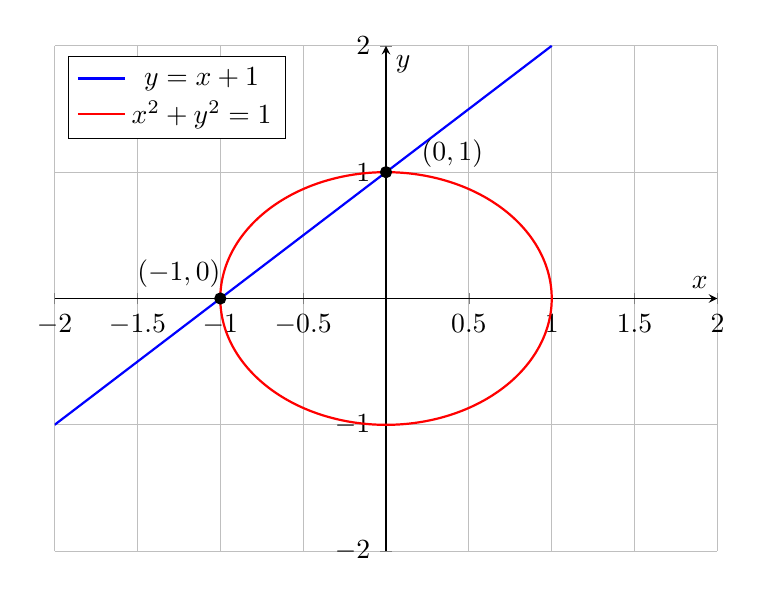
\begin{tikzpicture}
\begin{axis}[
axis lines=middle,
xmin=-2,
xmax=2,
ymin=-2,
ymax=2,
grid=major,
width=10cm,
height=8cm,
xlabel=$x$,
ylabel=$y$,
legend style={
at={(0.02,0.98)},
anchor=north west
}
]

% đường thẳng
\addplot[
blue,
thick,
domain=-2:1
]
{x+1};

% đường tròn
\addplot[
red,
thick,
samples=300,
domain=0:360
]
({cos(x)},{sin(x)});

% giao điểm
\addplot[
only marks,
mark=*,
mark size=2pt
]
coordinates{
(-1,0)
(0,1)
};

\node at (axis cs:-1.25,0.2) {$(-1,0)$};
\node at (axis cs:0.4,1.15) {$(0,1)$};

\legend{$y=x+1$,$x^2+y^2=1$}

\end{axis}
\end{tikzpicture}
\end{center}

Quan sát hình vẽ, hai đồ thị cắt nhau tại:

\[
(-1,0),\ (0,1)
\]

Vậy hệ có hai nghiệm:

\[
\boxed{(-1,0)\text{ và }(0,1)}
\]
Trong đó đường màu xanh dương chính là đồ thị của phương  $x+1-y=0$
và đường màu đỏ là đồ thị của phương trình $x^2+y^2=1$.

\end{vd}


\begin{nx}
    \begin{itemize}
\item Phương pháp biểu diễn hình học giúp đưa ra hình ảnh trực quan về nghiệm của hệ phương trình thông qua việc biểu diễn các phương trình dưới dạng đồ thị trên cùng một hệ trục tọa độ.
    
    \item Giúp người học nhận thấy rõ mối quan hệ giữa nghiệm của hệ phương trình và giao điểm của các đồ thị; từ đó dễ dàng xác định số nghiệm của hệ.
    
    \item Tạo điều kiện thuận lợi trong việc dự đoán nghiệm và hỗ trợ quá trình phân tích bài toán theo hướng trực quan.
    
    \item Tuy nhiên, phương pháp này gặp khó khăn khi áp dụng cho hệ phương trình có từ ba ẩn trở lên; đặc biệt đối với hệ nhiều ẩn thì việc biểu diễn hình học gần như không khả thi.
    
    \item Việc xác định nghiệm bằng đồ thị thường chỉ mang tính gần đúng, do đồ thị chủ yếu cho biết sự tồn tại của giao điểm và vị trí tương đối của nghiệm, khó xác định chính xác tọa độ.
    
    \item Đối với các hàm số có đồ thị phức tạp hoặc khó vẽ, việc áp dụng phương pháp này có thể gặp nhiều trở ngại nếu không có sự hỗ trợ của các phần mềm toán học.
    
    \item Vì vậy, phương pháp biểu diễn hình học phù hợp để minh họa, hỗ trợ trực quan và định hướng lời giải; tuy nhiên cần kết hợp với các phương pháp đại số để xác định nghiệm chính xác.
    \end{itemize}
\end{nx}
\subsection{Phương pháp sử dụng tính đơn điệu của hàm số}
    \subsubsection{Phương pháp giải:}
    Phương pháp này áp dụng tính chất một hàm số $f$ liên tục, đơn điệu trên một khoảng nếu $f(x)=0$ có nghiệm thì nghiệm đó là duy nhất. Hơn thế nữa, $f(a)=f(b) $ khi và chỉ khi $a=b$. 
    \begin{enumerate}
        \item Cố gắng tìm một nghiệm của hệ phương trình ban đầu.
        \item Xây dựng một hàm số sao cho hàm có tính đơn điệu và liên tục trên khoảng cần xét.
        \item Sử dụng tính đơn điệu để chứng minh nghiệm duy nhất của hệ phương trình.
    \end{enumerate}
   \begin{vd} Giải hệ phương trình:

\[
\begin{cases}
\sqrt{x+2}+\sqrt{x+4}
=
\sqrt{y-2}+\sqrt{y-4}\\
x^2+y^2+x+y=32
\end{cases}
\]

\textbf{Lời giải.}

Đầu tiên ta tìm điều kiện xác định của hệ phương trình là:
\[x\ge -2;\qquad y\ge 4.
\]
Xét phương trình thứ nhất:
\[
\sqrt{x+2}+\sqrt{x+4}
=\sqrt{y-2}+\sqrt{y-4}.
\]
Thay \(x=y-6\) vào hệ ta thấy:
\[
\sqrt{y-4}+\sqrt{y-2}
=\sqrt{y-2}+\sqrt{y-4},
\]
suy ra VT = VP.
Xét hàm số
\[
f(t)=\sqrt{t+2}+\sqrt{t+4},
\]
ta có \(f(t)\) đồng biến trên miền xác định.
Với \(x>y-6\) thì \(f(x)>f(y-6)\), suy ra VT \(>\) VP; ngược lại với \(x<y-6\) thì VT \(<\) VP.
Do đó:
\[x=y-6\]
là phương trình tương đương của phương trình thứ nhất.
Thay vào phương trình thứ hai ta được:
\[
(y-6)^2+y^2+y-6+y=32
\]
\[
\Leftrightarrow
2y^2-10y-2=0
\]
\[
\Leftrightarrow y^2-5y-1=0\]
\[\Leftrightarrow
\left[
\begin{aligned}
y&=\dfrac{5+\sqrt{29}}{2}\\
y&=\dfrac{5-\sqrt{29}}{2}\quad (\text{loại})
\end{aligned}
\right.\]
Do điều kiện \(y\ge4\), nhận:
\[y=\dfrac{5+\sqrt{29}}{2}.
\]
Khi đó:
\[x=y-6=\dfrac{\sqrt{29}-7}{2}.\]
Vậy nghiệm của hệ phương trình ban đầu là:
\[
\boxed{
\left(
\dfrac{\sqrt{29}-7}{2},
\dfrac{5+\sqrt{29}}{2}
\right)
}
\]
\end{vd}
    \begin{nx}
        \begin{itemize}
            \item Đây là một phương pháp thông qua việc đánh giá nghiệm của ẩn và điểm chung của một phương trình để đưa về hàm số liên tục và sử dụng tính đơn điệu để chứng minh duy nhất nghiệm.
            \item Phương pháp này áp dụng được đa dạng hệ phương trình và phương trình tuy nhiên khi sử dụng phải nhớ điều kiện liên tục của hàm số.
            \item Việc đánh giá và chọn hàm là tùy theo ý tưởng giải quyết bài toán, không cố định.
        \end{itemize}
    \end{nx}
    \subsection{Phương pháp sử dụng bất đẳng thức} 
    \subsubsection{Phương pháp giải:}
    Thông thường phương pháp được sử dụng với những hệ phương trình có số phương trình ít hơn số ẩn. Tuy nhiên có những hệ số phương trình bằng số ẩn cũng có thể sử dụng phương pháp này. Có hai cách làm chủ yếu:
    \begin{enumerate}
        \item  Cố gắng tìm một nghiệm "đẹp" của hệ phương trình. Chứng minh nghiệm đó là duy nhất bằng cách xét những trường hợp khác giá trị đó và chứng minh những giá trị đó không là nghiệm. 
        \item Tìm mối quan hệ giữa các ẩn và các bất đẳng thức quen thuộc. Áp dụng tính chất "đẳng thức/dấu '=' xảy ra" của bất đẳng thức để suy ra nghiệm.
    \end{enumerate}


\begin{vd}
    \textbf{Ví dụ.} Giải hệ phương trình sau biết các giá trị trong nghiệm đều dương:

\[
\begin{cases}
x+y+z=12\\
(2+x)(2+y)(2+z)=\left(2+\sqrt[3]{xyz}\right)^3
\end{cases}
\]

\textbf{Lời giải.}

Áp dụng bất đẳng thức AM-GM:
\[x+y+z\ge 3\sqrt[3]{xyz}.\]
Do \(x+y+z=12\), suy ra:
\[4\ge \sqrt[3]{xyz}. \tag{1}
\]
Mặt khác:
\[xy+yz+zx\ge 3\sqrt[3]{(xyz)^2}. \tag{2}
\]
Xét phương trình thứ hai:
\begin{align*}
(2+x)(2+y)(2+z)
&=8+4(x+y+z)+2(xy+yz+zx)+xyz\\
&=56+2(xy+yz+zx)+xyz.
\end{align*}
Ta có:
\[
56=8+48.
\]
Từ (1):
\[48\ge 12\sqrt[3]{xyz},
\]
và từ (2):
\[2(xy+yz+zx)\ge 6\sqrt[3]{(xyz)^2}.
\]
Do đó:
\begin{align*}
(2+x)(2+y)(2+z)
&\ge 8+12\sqrt[3]{xyz}
+6\sqrt[3]{(xyz)^2}+xyz\\
&=\left(2+\sqrt[3]{xyz}\right)^3.
\end{align*}
Dấu bằng xảy ra khi:
\[x=y=z.
\]
Thế vào \(x+y+z=12\) ta được:
\[3x=12\Rightarrow x=4.
\]
Vậy hệ có nghiệm:
\[
\boxed{(4;4;4)}.
\]
\end{vd}
   

    \begin{nx}
        \begin{itemize}
    \item Việc xét điều kiện xảy ra dấu bằng của bất đẳng thức giúp xác định nghiệm nhanh và hiệu quả.
    \item Tuy nhiên, phương pháp này phụ thuộc nhiều vào khả năng lựa chọn bất đẳng thức phù hợp.
    \item Trong một số trường hợp, việc áp dụng bất đẳng thức có thể khó định hướng và không có quy trình giải cố định.
\end{itemize}
    \end{nx}

   \chapter{MỘT SỐ HỆ PHƯƠNG TRÌNH ĐẠI SỐ VÀ PHƯƠNG PHÁP GIẢI}
    \section{Hệ phương trình tuyến tính}
    \subsection{Một số định nghĩa}
    \begin{dn}
      Cho $m, n$ là các số nguyên dương. \textit{Hệ phương trình tuyến tính cấp $m \times n$} trên trường $\mathbb{K}$ là một tập các phương trình có dạng
\begin{equation} 
\left\{
\begin{array}{lcl}
a_{11}x_1 + a_{12}x_2 + \cdots + a_{1n}x_n &=& b_1 \\
a_{21}x_1 + a_{22}x_2 + \cdots + a_{2n}x_n &=& b_2 \\
\cdots \quad \cdots \quad \cdots \quad \cdots \quad \cdots && \cdots \\
a_{m1}x_1 + a_{m2}x_2 + \cdots + a_{mn}x_n &=& b_m \\
\end{array}
\right.
\end{equation}
trong đó $a_{ij}, b_i \in \mathbb{K}$ với mọi $i = 1, \dots, m$ và $j = 1, \dots, n$. Các số $a_{ij} \in \mathbb{K}$ được gọi là các \textit{hệ số}, còn các số $b_1, \dots, b_m$ được gọi là các \textit{hệ số tự do}, và $x_1, \dots, x_n$ được gọi là các \textit{ẩn} của hệ phương trình tuyến tính.
    \end{dn}
\begin{dn}
    Cho $m, n$ là các số nguyên dương. Một \textbf{ma trận} cấp $m \times n$ là một bảng số hình chữ nhật gồm $mn$ số $a_{ij} \in \mathbb{K}$ ($i = 1, \ldots, m;\ j = 1, \ldots, n$) được xếp thành $m$ dòng và $n$ cột
\[
\begin{bmatrix}
a_{11} & a_{12} & \cdots & a_{1n} \\
a_{21} & a_{22} & \cdots & a_{2n} \\
\vdots & \vdots & \ddots & \vdots \\
a_{m1} & a_{m2} & \cdots & a_{mn}
\end{bmatrix}.
\]

Các số $a_{ij}$ nằm ở dòng thứ $i$ và cột thứ $j$ được gọi là các phần tử của ma trận. Người ta thường ký hiệu cho ma trận bởi các chữ in hoa $A, B, C, \ldots$ Một ma trận $A$ cấp $m \times n$ thường được viết gọn dạng $A = (a_{ij})_{m \times n}$.
\end{dn}
\begin{nx}
   
         Với hệ phương trình tuyến tính 
        
        \begin{equation} 
\left\{
\begin{array}{lcl}
a_{11}x_1 + a_{12}x_2 + \cdots + a_{1n}x_n &=& b_1 \\
a_{21}x_1 + a_{22}x_2 + \cdots + a_{2n}x_n &=& b_2 \\
\cdots \quad \cdots \quad \cdots \quad \cdots \quad \cdots && \cdots \\
a_{m1}x_1 + a_{m2}x_2 + \cdots + a_{mn}x_n &=& b_m \\
\end{array}
\right.
\end{equation}
 \begin{itemize}
 \item Ma trận
\[A \;=\;
\begin{bmatrix}
a_{11} & a_{12} & \cdots & a_{1n} \\
a_{21} & a_{22} & \cdots & a_{2n} \\
\vdots & \vdots & \ddots & \vdots \\
a_{m1} & a_{m2} & \cdots & a_{mn}
\end{bmatrix}.
\] được gọi là \textit{ma trận hệ số} của hệ phương trình $(2.1.2)$.

\item Ma trận 
\[\bar{A} \;=\;
\left[\begin{array}{cccc|c}
a_{11} & a_{12} & \cdots & a_{1n} & b_1 \\
a_{21} & a_{22} & \cdots & a_{2n} & b_2\\
\vdots & \vdots & \ddots  & \vdots & \vdots \\
a_{m1} & a_{m2} & \cdots & a_{mn} & b_n
\end{array}\right].
\] được gọi là \textit{ma trận mở rộng} của hệ phương trình $(2.1.2)$ hay có thể viết dưới dạng $\bar{A}=[A,b]$, trong đó $b=[b_1,b_2,...b_n]^T$ là cột hệ số tự do của hệ phương trình.
\item Với một hệ phương trình tuyến tính khi giải nghiệm thì thực chất là đang làm việc với những hệ số do đó một số phép biến đổi tương đương: thay đổi vị trí các phương trình, nhân một phương trình với hệ số khác $0$, cộng các phương trình với nhau sẽ tương ứng với các phép biến đổi sơ cấp của ma trận: đổi vị trí các dòng, nhân một dòng của ma trận với hệ số khác $0$, cộng các dòng của ma trận với nhau. 
\item Nếu xét trong không gian Afin $\mathbb{A}^n$ thì mỗi phương trình của hệ phương trình tuyến tính cho ta một siêu phẳng và nghiệm của hệ phương trình chính là phần giao của các siêu phẳng.

\begin{vd}
    
Xét không gian Euclid $\mathbb{R}^3$, nghiệm của hệ phương trình tuyến tính

\begin{equation}
\left\{
\begin{array}{lcl}
x+y-z=0\\
x+y=3\\
2x-y=0
\end{array}
\right.
\end{equation} 

chính là tọa độ giao điểm của $3$ mặt phẳng $x+y-z=0,  
 x+y=3,
 2x-y=0.$

\begin{figure}[h]
    \centering
    \includegraphics[width=0.9\textwidth]{z7861351831941_c3209589aa8fb088df9dca2e786df9d4.jpg}
    \caption{Biễu diễn hệ phương trình trong không gian $3$ chiều}
    \label{fig:enter-label}
\end{figure}

    Dựa vào hình ảnh ta cũng thấy được rằng nghiệm của hệ phương trình là giao của $3$ mặt phẳng chính là một điểm và tọa độ điểm đó là $(2;1;5)$. 

    Và khi giải bằng các phương pháp sử dụng phép biến đổi tương đương thì cho ra được nghiệm của hệ phương trình là $A(2;1;5)$.
    \end{vd} 
    \end{itemize}
    \end{nx}
    Đối với hệ phương trình tuyến tính ta có thể giải bằng nhiều phương pháp như dùng phương pháp thế, phương pháp cộng đại số, phương pháp sử dụng các phép biến đổi tương đương, biểu diễn hình học, v.v. những phương pháp này đã được đề cập ở \textbf{Chương 1} nên ở phần này chỉ tập trung vào những phương pháp khác chưa được đề cập.
\subsection{Phương pháp sử dụng ma trận - Sử dụng các phép biến đổi sơ cấp}
\subsubsection{Phương pháp giải:}
Cho hệ phương trình tuyến tính cấp $m \times n$ như sau
\begin{equation} 
\left\{
\begin{array}{lcl}
a_{11}x_1 + a_{12}x_2 + \cdots + a_{1n}x_n &=& b_1 \\
a_{21}x_1 + a_{22}x_2 + \cdots + a_{2n}x_n &=& b_2 \\
\cdots \quad \cdots \quad \cdots \quad \cdots \quad \cdots && \cdots \\
a_{m1}x_1 + a_{m2}x_2 + \cdots + a_{mn}x_n &=& b_m \\
\end{array}
\right.
\end{equation}
\begin{enumerate}
    \item Xét ma trận mở rộng $A=[(a_{ij})_{m \times n},\vec{b}]$ của hệ phương trình 
    
    Trong đó $\vec{b}=[b_1,b_2,...b_n]^T$ là cột hệ số tự do của hệ phương trình.
    \item Dùng phương pháp khử Gauss-Jordan để đưa ma trận $A$ về ma trận bậc thang hay ma trận bậc thang rút gọn.
    \item Đưa lại về dạng hệ phương trình để tìm nghiệm.
\end{enumerate}

\begin{vd}
Giải hệ phương trình sau: \begin{equation}
\left\{
\begin{array}{lcl}
x + 2y +3z &=&1 \\
y+z&=&1 \\
x+y+z &=&0 
\end{array}
\right.
\end{equation}

\textbf{\textit{Lời giải.}}   

Xét ma trận mở rộng $\bar{A}$ của $(2.1.5)$ ta được:
\begin{align*}
\bar{A}=\left[
\begin{array}{lcl|c}
1 & 2&3 &1 \\
0&1&1&1 \\
1&1&1 &0 
\end{array}
\right]&\xrightarrow[]{-d_3+d_1}\left[
\begin{array}{lcl|c}
1 & 2&3 &1 \\
0&1&1&1 \\
0&1&2 &1 
\end{array}
\right]\xrightarrow[]{d_3-d_2}\left[
\begin{array}{lcl|c}
1 & 2&3 &1 \\
0&1&1&1 \\
0&0&1 &0 
\end{array}
\right]\\&\xrightarrow[d_2-d_3]{d_1-2d_2-d_3}\left[
\begin{array}{lcl|c}
1 & 0&0 &-1 \\
0&1&0&1 \\
0&0&1 &0 
\end{array}
\right]\end{align*}

Khi đó hệ phương trình của ta tương đương hệ phương trình
\[\left\{
\begin{array}{lcl}
x  &=&-1 \\
y&=&1 \\
z&=&0
\end{array}
\right.\]

Vậy hệ ban đầu có nghiệm $(-1;1;0)$.
\end{vd}

\begin{nx}
\begin{itemize}
    \item  Một hệ phương trình cấp $m\times n$ có thể được viết dưới dạng 
    $A\vec{x}=\vec{b} $ trong đó $A=(a_{ij})_{m\times n} $ là ma trận hệ số của hệ phương trình đã cho, $\vec{x}=[x_1,x_2,...,x_n]^T$ là ẩn của hệ phương trình, $\vec{b}=[b_1,b_2,...,b_n]^T$ là hệ số tự do của hệ phương trình.
    \item Nếu hệ phương trình có cấp là $n\times n$ khi đó ma trận hệ số $A$ của hệ phương trình là ma trận vuông cấp $n\times n$. Hơn nữa nếu $A$ khả nghịch thì hệ phương trình ban đầu có nghiệm duy nhất $\vec{x}=A^{-1}\vec{b}$.

    \item Ngoài ra ta có thể kết luận nghiệm của hệ phương trình thông qua ma trận hệ số của hệ đó khi đưa về dạng ma trận bậc thang như sau:
    \begin{itemize}
        \item Nếu $rank(A)< rank(\bar{A})$ thì hệ phương trình vô nghiệm.
        \item Nếu $rank(A)= rank(\bar{A})=n$ thì hệ phương trình có một nghiệm duy nhất.
        \item Nếu $rank(A)= rank(\bar{A})=r<n$ thì hệ phương trình có vô số nghiệm và nghiệm tổng quát của hệ có $r$ ẩn phụ thuộc vào $n-r$ ẩn tự do.
    \end{itemize}
    
\end{itemize}
\end{nx}

\subsection{Phương pháp sử dụng định thức - Quy tắc Cramer}
\subsubsection{Quy tắc Cramer:}
     Hệ phương trình tuyến tính cấp $n\times n$ trên trường $\mathbb{K}$ có dạng 
    \begin{equation}
        A\vec{x}=\vec{b}
    \end{equation} trong đó:
\begin{itemize}
    \item $A=(a_{ij})_n\neq0$ là ma trận hệ số của hệ phương trình $(2.1.6)$.
    \item $\vec{x}=[x_1,x_2,...,x_n]^T$ là ma trận (cột) ẩn của hệ phương trình $(2.1.6)$.
    \item $\vec{b}=[b_1,b_2,...,b_n]^T$ là ma trận (cột) hệ số tự do của hệ phương trình $(2.1.6)$.
    
    \end{itemize}
    
    Nếu $\det{A}\neq 0$ thì hệ phương trình $(2.1.6)$ có nghiệm $\vec{x}=[x_1,x_2,...,x_n]^T$ với các thành phần $x_i$ được tính bởi

   \[
x_i = \frac{\det A_i(\vec{b})}{\det A} \hspace{1cm} i=1;2;...;n
\]

Với $ A_i(\vec{b})$ là ma trận $A$ nhưng thay cột thứ $i$ bằng ma trận cột $\vec{b}$.
\begin{nx}
    Nếu $\det{A}= 0$ thì có hai trường hợp xảy ra như sau:
    \begin{itemize}
        \item Nếu $\forall i=1;2;...n: \det A_i(\vec{b})=0 $ thì hệ phương trình $(2.1.5)$ có vô số nghiệm.
        \item Nếu $\exists i\in \{1;2;...;n\}:\det A_i(\vec{b})\neq0  $ thì hệ phương trình $(2.1.5)$ vô nghiệm.
     \end{itemize}
\end{nx}
\begin{vd}
    Giải hệ phương trình sau bằng quy tắc Cramer:
    
\begin{equation}
\left\{
\begin{array}{lcl}
x + 2y +z  &=& 2 \\
2x+y-4z &=& 1 \\
2x+y+2z &=& 2 \\
\end{array}
\right.
\end{equation}

\textbf{\textit{Lời giải.}}

Ta xét ma trận hệ số của hệ phương trình $(2.1.7)$ là 
\[A \;=\;
\begin{bmatrix}
1 &2 & 1  \\
2 & 1 & -4 \\
2 & 1& 2
\end{bmatrix}\]
và cột hệ số tự do \[\vec{b} \;=\;
\begin{bmatrix}
2\\1\\2
\end{bmatrix}\]
Ta có: \begin{align*}
    & \det A=-18\neq0\\
    & \det A_x(\vec{b}) \;=\;
\begin{vmatrix}
2 &2 & 1  \\
1 & 1 & -4 \\
2 & 1& 2
\end{vmatrix}=-9\\
    & \det A_y(\vec{b}) \;=\;
\begin{vmatrix}
1 &2 & 1  \\
2 & 1 & -4 \\
2 & 2& 2
\end{vmatrix}=-12\\
    &\det A_z(\vec{b}) \;=\;
\begin{vmatrix}
1 &2 & 2  \\
2 & 1 & 1 \\
2 & 1& 2
\end{vmatrix}=-3\\
\end{align*}


Theo quy tắc Cramer thì ta có nghiệm của hệ phương trình là $(x,y,z)$ với

\begin{align*}
    & \displaystyle x=\frac{\det A_x(\vec{b})}{\det A}=\frac{1}{2}\\
    & \displaystyle y=\frac{\det A_y(\vec{b})}{\det A}=\frac{2}{3}\\
    & \displaystyle z=\frac{\det A_z(\vec{b})}{\det A}=\frac{1}{6}
\end{align*}

Vậy hệ phương trình $(2.1.7)$ có một nghiệm duy nhất là $\left(\displaystyle \frac{1}2,\frac{2}3,\frac{1}6\right)$.
\end{vd}
    
Bên cạnh các phương pháp kể trên, để giải quyết một hệ phương trình tuyến tính còn có nhiều phương pháp khác trong đại số tuyến tính và các ngành cơ sở dữ liệu, tiêu biểu như:
 Phương pháp phân tích LU (LU Decomposition), phương pháp Jacobi - Gauss-Seidel, phương pháp QR (QR Decomposition), phương pháp phân tích giá trị kì dị (SVD - Singular Value Decomposition), v.v.  

\section{Hệ phương trình phi tuyến tính thường gặp}
Hệ phương trình phi tuyến tính là những hệ mà trong đó các phương trình không còn tuân theo dạng tuyến tính tổng quát 
$a_1x_1+a_2x_2+...+a_nx_n=b$ như đã nêu ở phần trước. Do sự xuất hiện của các biểu thức phi tuyến như tích các ẩn, căn thức, phân thức, hoặc các hàm mũ bậc cao, loại hệ này đa dạng về hình thức và thường có tính chất phức tạp hơn đáng kể so với hệ tuyến tính.

Chính vì tính chất phi tuyến và độ phức tạp tăng cao, việc giải hệ phương trình phi tuyến (đặc biệt là những hệ có cấp cao hoặc chứa nhiều ẩn) thường khó thực hiện bằng các phương pháp giải thông thường và trong nhiều trường hợp đòi hỏi phải sử dụng đến các công cụ tính toán hỗ trợ hoặc phương pháp giải gần đúng.

Trong phạm vi tiểu luận này, nội dung sẽ tập trung trình bày một số dạng tiêu biểu của hệ phương trình phi tuyến tính, chủ yếu là các hệ hai ẩn và ba ẩn, nhằm làm rõ phương pháp tiếp cận và cách giải quyết các dạng bài toán điển hình thuộc loại hệ này.
\subsection{Hệ phương trình chứa tích các ẩn}
\subsubsection{Đặc điểm nhận biết:} Hệ phương trình chứa tích các ẩn là hệ phương trình có ẩn là $x=(x_1;x_2;...x_n)$ mà trong đó các phương trình có chứa tích của các ẩn dạng $\displaystyle \prod_{i\in I}{x_i}, I \subset \{1;2;...;n\}$.
\subsubsection{Phương pháp giải:} Các bài toán hệ phương trình chứa tích các ẩn sẽ có nhiều phương pháp giải khác nhau: 
\begin{itemize}
    \item Đối với bài toán hệ phương trình $2$ ẩn, $3$ ẩn xuất hiện tổng hoặc tích các ẩn như $x+y+z$, $xy+xz+yz$, $xyz$ (biểu diễn nghiệm của đa thức bậc $3$) hay $x+y$, $xy$ (biểu diễn nghiệm của đa thức bậc $2$) thì ta sẽ đặt ẩn phụ theo các cụm đó và dùng định lí Vi-ét để đưa về dạng nghiệm của phương trình bậc tương ứng để giải quyết.
    \item Ngoài ra sử dụng phương pháp thế để giải quyết cũng là một phương án hữu hiệu nếu bài toán không quá phức tạp hoặc bài toán không thể định dạng thông qua định lí Vi-ét.
\end{itemize}
\begin{vd}
    Giải hệ phương trình sau
     \begin{equation} \left\{ \begin{aligned} x+y &= 5\\ xy &= 6 \end{aligned} \right. \end{equation}
\bigskip
\textbf{Lời giải.}
\medskip
\textbf{Cách 1: Đặt ẩn phụ}

Đặt
\[
\left\{
\begin{aligned}
S&=x+y\\
P&=xy
\end{aligned}
\right.
\]
Theo định lí Vi-ét đảo, \(x,y\) là các nghiệm của phương trình bậc hai
\[X^2-SX+P=0
\]
Thay \(S=5,\ P=6\), ta được
\[
X^2-5X+6=0 \qquad (*)
\]

Ta có
\[
X^2-5X+6=(X-2)(X-3)=0
\]

Suy ra phương trình \((*)\) có hai nghiệm là \(2\) và \(3\).

Do đó
\[
x,y\in\{2;3\}
\]

Với \(x=2\) thì \(y=3\).

Với \(x=3\) thì \(y=2\).

Vậy hệ phương trình có hai nghiệm:
\[
(2;3),\ (3;2)
\]

\bigskip

\textbf{Cách 2: Sử dụng phương pháp thế}

\[
\left\{
\begin{aligned}
x+y&=5\\
xy&=6
\end{aligned}
\right.
\]

\[
\Leftrightarrow
\left\{
\begin{aligned}
x&=5-y\\
(5-y)y&=6
\end{aligned}
\right.
\]

\[
\Leftrightarrow
\left\{
\begin{aligned}
5y-y^2&=6
\end{aligned}
\right.
\]
\[
\Leftrightarrow
y^2-5y+6=0
\]
\[
\Leftrightarrow
(y-2)(y-3)=0
\]
\[
\Leftrightarrow
\left[
\begin{aligned}
y&=2\\
y&=3
\end{aligned}
\right.
\]

Nếu \(y=2\) thì \(x=3\).

Nếu \(y=3\) thì \(x=2\).

Vậy hệ phương trình có nghiệm:
\[
(2;3),\ (3;2)
\]
\end{vd}

\begin{vd}
    Giải hệ phương trình sau: \begin{equation}
\left\{
\begin{array}{lcl}
x + y +z &=&6 \\
xy +yz+xz&=&11 \\
xyz &=&6
\end{array}
\right.
\end{equation}

\textbf{\textit{Lời giải.}}

Đặt $
\left\{
\begin{array}{lcl}
S &=& x + y +z \\
T&=&xy +yz+xz \\
 P&=&xyz
\end{array}
\right.$

Theo định lí Vi-ét đảo ta có $x,y,z$ là nghiệm của phương trình bậc ba \[X^3-SX^2+TX-P=0\Leftrightarrow X^3-6X^2+11X-6=0\]

Mà phương trình $X^3-6X^2+11X-6=0$ có ba nghiệm là $X=1;X=2;X=3$.

Nên $x,y,z \in \{1;2;3\}$.

Với $x=1$ thay vào $(2.2.10)$ ta được hệ mới như sau
\[\left\{
\begin{array}{lcl}
y+z &=& 5 \\
y+z+yz&=&11 \\
 yz&=&6
\end{array}
\right.\Leftrightarrow\left\{
\begin{array}{lcl}
y+z &=& 5 \\
 yz&=&6
\end{array}
\right.\]

Giải tiếp tục như \textbf{Ví dụ 2.2.1} ta được $(y,z)=(2;3)$ và $(y,z)=(2;3)$.

Do đó ta được hai nghiệm của $(2.2.9)$ là $(1;2;3)$ và $(1;3;2)$.

Với $x=2$ ta giải được hai nghiệm của $(2.2.9)$ là $(2;1;3)$ và $(2;3;1)$.

Với $x=3$ ta giải được hai nghiệm của $(2.2.9)$ là $(3;1;2)$ và $(3;2;1)$.

Vậy hệ phương trình $(2.2.9)$ có sáu nghiệm là $(1;2;3)$, $(1;3;2)$, $(2;1;3)$, $(2;3;1)$, $(3;1;2)$, $(3;2;1)$.
\end{vd}

\begin{nx}
    Khi giải hệ phương trình hai (hoặc ba ẩn) dạng chứa tích các ẩn ta luôn tìm cách biểu diễn chúng thành dạng có thể đưa về phương trình bậc hai (hoặc ba) thông qua định lí Vi-ét. 
    \begin{itemize}
        \item Nếu biểu diễn được dưới dạng đó thì ta sẽ luôn có bộ số $(x,y)$ hoặc $(x,y,z)$ chính là hoán vị các nghiệm của phương trình bậc tương ứng khi biểu diễn thông qua định lí Vi-ét.
        \item Nếu ta không thể biểu diễn được dưới dạng đó thì sử dụng phương pháp thế tuy nhiên đổi với phương pháp thế có thể khiến bài toán trở nên phức tạp.
        
    \end{itemize}
\end{nx}
  \subsection{Hệ phương trình chứa ẩn ở mẫu}
\subsubsection{Đặc điểm nhận biết:}
Một hệ phương trình mà trong đó các phương trình có chứa phân thức hay ẩn của phương trình nằm dưới mẫu thì được gọi là hệ phương trình chứa ẩn ở mẫu.
\subsubsection{Phương pháp giải:} Thông thường những bài toán hệ phương trình có chứa ẩn ở mẫu sẽ được giải theo phương pháp đặt ẩn phụ để đổi biến (kèm điều kiện) đưa về hệ phương trình không còn có chứa ẩn ở mẫu hoặc vẫn chứa nhưng có thể giải được để giải quyết. Có thể làm theo các bước sau:
\begin{enumerate}
    \item Đặt điều kiện xác định của các phương trình.
    \item Đổi biến kèm điều kiện của biến. Giải hệ phương trình với hệ ẩn mới.
    \item Thay các ẩn vừa tìm được vào phần đặt để giải ra các ẩn ban đầu.
    \item Kiểm tra lại các giá trị vừa tìm có là nghiệm hay không trong trường hợp các phép biến đổi không tương đương. 
\end{enumerate} 
\begin{vd}
  Giải hệ phương trình sau:
    \begin{equation}
\left\{
\begin{array}{lcl}
\displaystyle \frac{1}{2x-1} + \frac{3}{y} +\frac{1}{z+1} &=& 3 \\[1.5ex]
\displaystyle \frac{1}{2x-1}+ \frac{3y+2z+2}{zy+y}&=&1 \\[1.5ex]
\displaystyle \frac{2x+y-1}{(2x-1)y} -\frac{z}{z+1}&=&0
\end{array}
\right.
\end{equation}

\textbf{\textit{Lời giải.}}

  Ta thấy mẫu của các phân thức trong hệ này đều chứa $2x-1$, $y$ và $z+1$  chúng ta tách thành các phân thức rời nhau với mẫu là ba biểu thức đó.

    Điều kiện xác định của hệ phương trình là $x\neq \displaystyle\frac{1}2,y\neq0,z\neq-1$.
    
    Ở phương trình thứ hai ta biến đổi thành 
    \[
    \displaystyle \frac{1}{2x-1}+ \frac{3y+2z+2}{zy+y}=1 \Leftrightarrow \frac{1}{2x-1}+\frac{3y+2(z+1)}{y(z+1)}=1\Leftrightarrow \frac{1}{2x-1} +\frac{2}{y}+\frac{3}{z+1}=1
    \].

    Tiếp tục biến đổi phương trình thứ ba ta được
     \[
    \displaystyle \frac{2x+y-1}{(2x-1)y} -\frac{z}{z+1}=0\Leftrightarrow \frac{1}{2x-1}+\frac{1}{y}+ \frac{1}{z+1}=1
    \].

    
Khi đó:
$(2.2.10)\Leftrightarrow\left\{
\begin{array}{lcl}
\displaystyle \frac{1}{2x-1} + \frac{3}{y} +\frac{1}{z+1} &=& 3 \\[1.5ex]
\displaystyle \frac{1}{2x-1} +\frac{2}{y}+\frac{3}{z+1}&=&1 \\[1.5ex]
\displaystyle \frac{1}{2x-1}+\frac{1}{y}+ \frac{1}{z+1}&=&1
\end{array}
\right.$ 

Đặt $\left\{
\begin{array}{lcl}
 A &=&\displaystyle \frac{1}{2x-1} \\[1.5ex]
 B&=& \displaystyle \frac{1}{y}\\[1.5ex]
 C&=&\displaystyle  \frac{1}{z+1}
\end{array}
\right.$

Hệ phương trình ban đầu trở thành hệ phương trình tuyến tính
\[\left\{
\begin{array}{lcl}
 A+3B+C&=& 3\\
A+2B+3C&=&1 \\
 A+B+C&=&1
\end{array}
\right.\xrightarrow{\text{Dạng ma trận}}\left[
\begin{array}{ccc}
 1&3&1\\
1&2&3\\
 1&1&1
\end{array}
\right].\left[
\begin{array}{ccc}
 A\\
B\\
 C
\end{array}
\right]=\left[
\begin{array}{ccc}
 3\\
1\\
 1
\end{array}
\right]\]

Ta có: \[\left|
\begin{array}{ccc}
 1&3&1\\
1&2&3\\
 1&1&1
\end{array}
\right|=4\neq0\]

Do đó ma trận hệ số của hệ phương trình tuyến tính trên là khả nghịch nên nghiệm của hệ phương trình tuyến tính trên là 
\[
\left[
\begin{array}{ccc}
 A\\
B\\
 C
\end{array}
\right]=\left[
\begin{array}{ccc}
 1&3&1\\
1&2&3\\
 1&1&1
\end{array}
\right]^{-1}.\left[
\begin{array}{ccc}
 3\\
1\\
 1
\end{array}
\right]=\left[
\begin{array}{ccc}
 \displaystyle \frac{1}2\\
 \displaystyle 1\\
 \displaystyle -\frac{1}2
\end{array}
\right]\]

Thay $A,B,C$ bằng các biểu thức đã đặt ta có hệ sau
\[\left\{
\begin{array}{lclcl}
 \displaystyle \frac{1}{2x-1} &=&A&=&\displaystyle \frac{1}2\\[1.5ex]
 \displaystyle \frac{1}{y}&=& B&=&\displaystyle 1\\[1.5ex]
 \displaystyle  \frac{1}{z+1}&=&C&=&\displaystyle -\frac{1}2
\end{array}
\right.\Longleftrightarrow\left\{
\begin{array}{lclcl}
 x&=&\displaystyle \frac{3}2\\[1.5ex]
y&=&  \displaystyle 1\\[1.5ex]
 z&=&\displaystyle -3
\end{array}
\right.\]

Ta thấy $(x,y,z)$ thỏa mãn các điều kiện xác định của hệ phương trình và khi thay vào hệ ban đầu thì đúng là nghiệm của hệ.

Vậy nghiệm của hệ phương trình $(2.2.10)$ là $(x,y,z)=\displaystyle
\left(\frac{3}2;1;-3\right)$.
\end{vd}

 \section{Hệ phương trình đối xứng và tuần hoàn}
Trong toán học cũng như trong nhiều bài toán thực tiễn, tính đối xứng và tính
tuần hoàn thường xuất hiện như những quy luật đặc trưng phản ánh mối liên hệ
giữa các đại lượng. Nhờ các đặc điểm này, nhiều mô hình phức tạp có thể được
đơn giản hóa và biểu diễn dưới dạng dễ phân tích hơn.

Trong giải hệ phương trình, việc nhận biết cấu trúc đối xứng hoặc tuần hoàn
giúp phát hiện những quan hệ đặc biệt giữa các ẩn số. Từ đó, ta có thể lựa chọn
các phép biến đổi thích hợp, đặt ẩn phụ hoặc khai thác tính chất của hệ để rút
gọn bài toán và tìm nghiệm một cách hiệu quả hơn.

Bên cạnh việc hỗ trợ tính toán, các hệ phương trình đối xứng và tuần hoàn
còn góp phần thể hiện tính hài hòa và quy luật của toán học trong việc mô tả
các hiện tượng tự nhiên và các mô hình thực tế.

\subsection{Hệ phương trình đối xứng loại I}
\subsubsection{Đặc điểm nhận biết:} Hệ phương trình đối xứng loại I là hệ phương trình mà khi thay các nghiệm cho nhau ta được hệ không đổi. Thông thường có thể gặp hệ phương trình này với $2$ hoặc $3$ ẩn.
\subsubsection{Phương pháp giải:}
\begin{enumerate}
    \item Đặt đổi biến:\begin{align*}
    &\text{Với hệ 2 ẩn}\left\{\begin{array}{lcl}
       S&=&x+y    \\
       P&=&xy  
    \end{array}\right.\\
      &\text{Với hệ 3 ẩn}\left\{\begin{array}{lcl}
       S&=&x+y+z  \\
       T&=&xy+yz+xz \\
       P&=&xyz  
    \end{array}\right.  \end{align*}
    \item Giải hệ phương trình với các ẩn $S,T,P$ vừa đặt.
    \item Sử dụng định lí Vi-ét để đưa về thành giải phương trình với số bậc tương ứng với số ẩn.
\end{enumerate}
\begin{vd}
     Giải hệ phương trình sau:
    \begin{equation}
\left\{
\begin{array}{lcl}
\displaystyle x+y+z&=&6 \\[1.5ex]
\displaystyle x^2+y^2+z^2&=&14\\[1.5ex]
\displaystyle x^3+y^3+z^3&=&36\\
\end{array}
\right.
 \end{equation}

 \textbf{\textit{Lời giải.}}

Ta có các phép biến đổi sau:
\begin{align*}
    &x^2+y^2+z^2=(x+y+z)^2-2(xy+yz+xz)\\
\Leftrightarrow&(xy+yz+xz)=\displaystyle\frac{1}2\left(-x^2-y^2-z^2+(x+y+z)^2\right)\\
\Leftrightarrow&(xy+yz+xz)=\displaystyle\frac{1}2\left(36-14\right)=11
\\
\\
&x^3+y^3+z^3=(x+y+z)^3-3(x+y+z)(xy+yz+xz)+3xyz\\
\Leftrightarrow&xyz=\displaystyle\frac{1}3\left(x^3+y^3+z^3-(x+y+z)^3+3(x+y+z)(xy+yz+xz)\right)\\
\Leftrightarrow&xyz=\displaystyle\frac{1}3\left(36-216+3.6.11\right)=6\end{align*}

Do đó hệ phương trình ban đầu của ta tương đương với hệ sau
\[\left\{
\begin{array}{lcl}
\displaystyle x+y+z&=&6 \\[1.5ex]
\displaystyle xy+z+xz&=&11\\[1.5ex]
\displaystyle xyz&=&6\\
\end{array}
\right.\]

Đặt $\left\{\begin{array}{lcl}
       S&=&x+y+z  \\
       T&=&xy+yz+xz \\
       P&=&xyz  
    \end{array}\right.$

Khi đó theo định lí Vi-ét đảo $x,y,z$ lần lượt là các nghiệm của phương trình bậc ba $X^3-SX^2+TX-P=0\Leftrightarrow X^3-6X^2+11X-6=0\Leftrightarrow\left[
\begin{array}{lcl}
\displaystyle X&=&\displaystyle 3\\[1.5ex]
\displaystyle X&=&\displaystyle 2\\[1.5ex]
\displaystyle X&=&\displaystyle 1
\end{array}
\right.$.

Vậy nghiệm của hệ phương trình $(2.3.11)$ là các hoán vị của bộ ba số \{1;2;3\}. 

Tức là $\{(x,y,z)|x,y,z\in\{1;2;3\}\}$.
\end{vd}

\begin{nx}\begin{itemize}
      \item Định lí Vi-ét giúp thể hiện mối quan hệ giữa phương trình bậc hai (ba) với hệ phương trình đối xứng với số ẩn tương ứng thông qua các biểu thức tính $S,T,P$.
      \item Do vai trò của các ẩn là giống nhau trong hệ đối xứng nên nghiệm của hệ phương trình loại này thường là các hoán vị các nghiệm của phương trình bậc tương ứng.
      \item Một số hệ phương trình cần phải qua vài bước biến đổi để đơn giản hóa bài toán và giúp dễ nhận dạng sau đó mới bắt đầu bước đặt.
      \item Hệ đẳng cấp bậc hai cũng là một trường hợp đặc biệt của hệ phương trình đối xứng loại I do đó việc ta khử ẩn $x^2$ hay khử ẩn $y^2$ là giống nhau và không mất tính tổng quát ta chỉ cần xét một biến $x$ hoặc $y$ khác 0 hoặc bằng 0 để giải là được. 
    \end{itemize}
\end{nx}

\subsection{Hệ phương trình đối xứng loại II}
\subsubsection{Đặc điểm nhận biết:} Hệ phương trình đối xứng loại II là hệ mà khi hoán vị (hoặc thay đổi) các ẩn theo một cách nào đó, thì các phương trình trong hệ cũng đổi vị trí tương ứng, nhưng toàn bộ hệ vẫn giữ nguyên (tức là không thay đổi về mặt tổng thể). Có thể mô tả qua công thức như sau:
\[\left\{
\begin{array}{lcl}
\displaystyle f(x,y)&=&a \\[1.5ex]
\displaystyle f(y,x)&=&a\\
\end{array}
\right.\]
\subsubsection{Phương pháp giải:} Với hệ phương trình có dạng
\[\left\{
\begin{array}{lcl}
\displaystyle f(x,y)&=&a \\[1.5ex]
\displaystyle f(y,x)&=&a\\
\end{array}
\right.\]

\begin{enumerate} 
    \item Dùng phương pháp cộng đại số đưa một phương trình của hệ về thành hiệu hai phương trình. Phương trình bị biến đổi có thể viết dưới dạng $(x-y)h(x,y)=0.$ 
\item Khi đó ta có được hai hệ phương trình mới là 
\[\left\{
\begin{array}{lcl}
\displaystyle f(x,y)&=&a \\[1.5ex]
\displaystyle x-y&=&0\\
\end{array}
\right.\hspace{10pt}\text{hoặc}\hspace{10pt}\left\{
\begin{array}{lcl}
\displaystyle f(x,y)&=&a \\[1.5ex]
\displaystyle h(x,y)&=&0\\
\end{array}
\right.\]
    \item Giải các hệ phương trình vừa có sau đó kiểm tra lại các nghiệm vừa tìm được có phải nghiệm của hệ phương trình ban đầu hay không.
\end{enumerate} 
\begin{vd}
     Giải hệ phương trình sau:
    \begin{equation}
\left\{
\begin{array}{lcl}
\displaystyle x^3-2y&=& -1\\[1.5ex]
\displaystyle y^3-2x&=&-1\\   
\end{array}
\right.
 \end{equation}

 \textbf{\textit{Lời giải.}}

Ta có: \[(2.3.21)\Leftrightarrow\left\{
\begin{array}{lcl}
\displaystyle x^3-2y&=& -1\\[1.5ex]
\displaystyle x^3-y^3+2(x-y)&=&0\\   
\end{array}
\right.\Leftrightarrow\left\{
\begin{array}{lcl}
\displaystyle x^3-2y&=& -1\\[1.5ex]
\displaystyle (x-y)\left(x^2+xy+y^2+2\right)&=&0\\   
\end{array}
\right.\] 

Khi đó ta có được hai hệ phương trình như sau:
\[\left\{
\begin{array}{lcl}
\displaystyle x^3-2y&=& -1\\[1.5ex]
\displaystyle x-y&=&0\\
\end{array}
\right.\hspace{10pt}\text{hoặc}\hspace{10pt}\left\{
\begin{array}{lcl}
\displaystyle x^3-2y&=&- 1\\[1.5ex]
\displaystyle x^2+xy+y^2+2&=&0\\
\end{array}
\right.\]

Xét hệ phương trình $\left\{
\begin{array}{lcl}
\displaystyle x^3-2y&=& -1\\[1.5ex]
\displaystyle x-y&=&0\\
\end{array}
\right.\Leftrightarrow\left\{
\begin{array}{lcl}
\displaystyle x^3-2y&=& -1\\[1.5ex]
\displaystyle x&=&y\\
\end{array}
\right.$

Thay $x=y$ vào phương trình đầu tiên ta được phương trình \[x^3-2x=-1 \Leftrightarrow(x-1)\left(x^2+x-1\right)=0\left[
\begin{array}{lcl}
\displaystyle x&=& 1\\[1.5ex]
\displaystyle x&=&\displaystyle\frac{-1+\sqrt{5}}2\\[1.5ex]
\displaystyle x&=&\displaystyle\frac{-1-\sqrt{5}}2
\end{array}
\right.\]

Thay lại vào hệ ta được ba nghiệm của hệ ban đầu là \[\displaystyle\left(1;1\right);\left(\displaystyle\frac{-1+\sqrt{5}}2;\displaystyle\frac{-1+\sqrt{5}}2\right);\left(\displaystyle\frac{-1-\sqrt{5}}2;\displaystyle\frac{-1-\sqrt{5}}2\right)\]

Xét hệ phương trình $\left\{
\begin{array}{lcl}
\displaystyle x^3-2y&=&- 1\\[1.5ex]
\displaystyle x^2+xy+y^2+2&=&0\\
\end{array}
\right.$
\end{vd}

Ở phương trình thứ hai $x^2+xy+y^2+2=0$ là một phương trình đối xứng bậc hai, ta xem đây là phương trình bậc hai theo ẩn là $x$ và $y$ là tham số. 

Ta tính $\Delta=y^2-4y^2-8=-3y^2-8<0$ do đó $x^2+xy+y^2+2=0$ vô nghiệm.

Nên trường hợp này hệ phương trình không có nghiệm.

Vậy nghiệm của hệ phương trình $(2.3.12)$ là
\[\displaystyle\left(1;1\right);\left(\displaystyle\frac{-1+\sqrt{5}}2;\displaystyle\frac{-1+\sqrt{5}}2\right);\left(\displaystyle\frac{-1-\sqrt{5}}2;\displaystyle\frac{-1-\sqrt{5}}2\right)\]

\subsection{Hệ phương trình hoán vị vòng quanh}
Khi mở rộng các hệ phương trình đối xứng loại II lên trường hợp có nhiều ẩn
hơn, ta thu được một dạng hệ phương trình đặc biệt gọi là hệ phương trình hoán
vị vòng quanh, hay còn được gọi ngắn gọn là hệ phương trình tuần hoàn.

Đặc trưng của dạng hệ này là các phương trình có cấu trúc tương tự nhau và
được tạo thành bằng cách hoán vị tuần tự vai trò của các ẩn số. Nhờ tính chất
lặp lại theo chu kì đó, ta có thể khai thác các mối liên hệ đối xứng giữa các ẩn
để đơn giản hóa việc giải hệ phương trình.

Trong nhiều trường hợp, việc nhận diện tính tuần hoàn giúp người giải dự đoán
được dạng nghiệm, thực hiện phép cộng hoặc trừ các phương trình tương ứng,
hay đưa hệ về các biểu thức quen thuộc để xử lí hiệu quả hơn.

\begin{dn}
    Hệ phương trình hoán vị vòng quanh là hệ phương trình mà nếu ta thực hiện một phép hoán vị vòng quanh các ẩn số (ví dụ: $x\to y, y \to z, z \to x$ đối với hệ ba ẩn), thì các phương trình trong hệ sẽ biến đổi thành nhau (hoặc giữ nguyên vị trí nếu hệ chỉ có một phương trình dạng $f(x,y,z) = f(y,z,x) = f(z,x,y))$.
    
Nói cách khác, nếu thay $x$ bởi $y$, $y$ bởi $z$, ..., ẩn cuối cùng bởi ẩn đầu tiên, thì hệ phương trình ban đầu sẽ thu được lại (có thể các phương trình đổi chỗ cho nhau).
\end{dn}
\subsubsection{Phương pháp giải:} Dạng tổng quát của hệ phương trình hoán vị vòng quanh là
\[\left\{
\begin{array}{lclcl}
\displaystyle f(x,y,z)&=& 0&(1)\\[1.5ex]
\displaystyle f(y,z,x)&=&0&(2)\\[1.5ex]
\displaystyle f(z,x,y)&=&0&(3)
\end{array}
\right.\]

Phương pháp giải hệ hoán vị vòng quanh thường dựa vào việc khai thác tính đối xứng của nó.
\begin{itemize}
    \item [\textit{Cách 1:}] Trừ vế theo vế.
    \begin{enumerate}
        \item Lấy phương trình $(1)$ trừ $(2)$, $(2)$ trừ $(3)$ và $(3)$ trừ $(1)$.
        \item Phân tích các phương trình thành nhân tử. Thông thường sẽ xuất hiện các nhân tử chung $(x-y), (y-z), (z-x)$.
        \item Xét trường hợp:
        
\textit{Trường hợp 1:} $x=y=z$. Thay điều kiện này vào một trong các phương trình ban đầu để giải phương trình một ẩn. Đây là trường hợp cho nghiệm phổ biến nhất.


\textit{Trường hợp 2:} $x,y,z$ không đồng thời bằng nhau. Giải các điều kiện còn lại từ bước 2.
    \end{enumerate}
    \item [\textit{Cách 2:}] Phương pháp đánh giá.
    \begin{enumerate}
        \item Giả sử tồn tại một thứ tự giữa các biến, ví dụ: $x\geq y\geq z$ (hoặc $x$ là biến lớn nhất, $x=\max\{x,y,z\}$).
        \item Từ giả thiết này và các phương trình của hệ, ta suy luận để tìm ra mối quan hệ tiếp theo giữa các biến.
        \item Thường thì quá trình suy luận sẽ dẫn đến kết luận mâu thuẫn (ví dụ $z\geq x$), hoặc kết luận duy nhất có thể xảy ra là $x=y=z$.
        \item  Giải trường hợp $x=y=z$ như \textit{Cách 1}.
    \end{enumerate}
\end{itemize}
\begin{vd}
Giải hệ phương trình sau:
    \begin{equation}
        \left\{
\begin{array}{lclcl}
\displaystyle x^2&=& 2y-1&(1)\\[1.5ex]
\displaystyle y^2&=&2z-1&(2)\\[1.5ex]
\displaystyle z^2&=&2x-1&(3)
\end{array}
\right.
    \end{equation}

\textbf{\textit{Lời giải.}}

Đầu tiên ta thấy tất cả vế trái đều là bình phương nên vế phải bắt buộc không âm tức là ta có điều kiện $x,y,z\ge \displaystyle\frac{1}2$.

Không mất tính tổng quát ta giả sử $x=\max\{x,y,z\}$, tức là $x\ge y,x\ge z$

Từ đây ta có: 
\begin{align*}\begin{array}{llclclclcl}
   2y-1=x^2\ge y^2=2z-1
   &\Leftrightarrow y\ge z\\
  &\Leftrightarrow y^2\ge z^2\\
   &\Leftrightarrow 2z-1\ge2x-1\\
   &\Leftrightarrow z\ge x
\end{array}
\end{align*}
Mà ta đang giả sử $x\ge z$ nên điều này chỉ xảy ra khi $z=x$ 
mà $x\ge y\ge z$ nên $x=y=z$.

Khi đó hệ phương trình ban đầu trở thành
\[\left\{
\begin{array}{lclcl}
\displaystyle x^2&=& 2x-1\\[1.5ex]
\displaystyle y^2&=&2y-1\\[1.5ex]
\displaystyle z^2&=&2z-1
\end{array}
\right.\Longleftrightarrow\left\{
\begin{array}{lclcl}
\displaystyle x&=& 1\\[1.5ex]
\displaystyle y&=&1\\[1.5ex]
\displaystyle z&=&1
\end{array}
\right.\]

Vậy hệ phương trình có nghiệm duy nhất là $(1;1;1)$.
\end{vd}


 \chapter{ỨNG DỤNG CỦA HỆ PHƯƠNG TRÌNH ĐẠI SỐ}
Trong toán học, hệ phương trình đại số là một công cụ quan trọng giúp mô tả
và làm rõ mối quan hệ giữa các đại lượng trong nhiều bài toán khác nhau. Việc
xây dựng và giải hệ phương trình không chỉ là một kĩ năng cơ bản của toán học
mà còn là phương tiện hữu hiệu để tiếp cận và giải quyết nhiều vấn đề trong
thực tiễn đời sống, khoa học và kĩ thuật.

Từ những bài toán đơn giản đến các mô hình phức tạp hơn, hệ phương trình
luôn giữ vai trò quan trọng trong việc biểu diễn các điều kiện ràng buộc giữa
các đại lượng. Thông qua việc chuyển đổi những tình huống thực tế thành các
mô hình toán học dưới dạng hệ phương trình, ta có thể phân tích, dự đoán và
tìm ra lời giải phù hợp cho bài toán đặt ra. Điều đó cho thấy tính ứng dụng rộng
rãi cũng như hiệu quả của tư duy toán học trong thực tế.

Nội dung chương này tập trung trình bày một số ứng dụng tiêu biểu của hệ
phương trình đại số thông qua các bài toán thực tiễn và mô hình toán học quen
thuộc. Qua đó, làm nổi bật vai trò của hệ phương trình trong việc ứng dụng toán
học vào đời sống, đồng thời thấy được giá trị và ý nghĩa thực tiễn mà chúng
mang lại.

\section{Lĩnh vực kinh tế}
\subsection{Bài toán: Mô hình kinh tế đầu vào - đầu ra Leontief}
\subsubsection{Mô tả bài toán:}
  Mô hình kinh tế đầu vào - đầu ra Leontief phân tích mối quan hệ phụ thuộc lẫn nhau giữa các ngành trong một nền kinh tế. Nó sử dụng một ma trận đầu vào - đầu ra để thể hiện lượng đầu vào từ một ngành cần thiết cho việc sản xuất của các ngành khác. Mục tiêu là xác định mức sản lượng mà mỗi ngành phải tạo ra để đáp ứng cả nhu cầu nội bộ giữa các ngành và nhu cầu cuối cùng của xã hội, giúp lập kế hoạch và phân tích tác động kinh tế.

  \begin{bt}
       Xét một hệ thống kinh tế đơn giản bao gồm ba ngành:
lúa gạo, dệt may và thép. Đầu ra của một đơn vị lúa gạo cần \(0,4\) đơn vị của
chính nó, \(0,2\) đơn vị dệt may và \(0,1\) đơn vị thép. Sản xuất một đơn vị dệt
may cần \(0,1\) đơn vị lúa gạo, \(0,5\) đơn vị của chính nó và \(0,2\) đơn vị thép.
Sản xuất một đơn vị thép cần \(0,2\) đơn vị lúa gạo, \(0,1\) đơn vị dệt may và
\(0,4\) đơn vị của chính nó.

\medskip

Giả sử hệ thống kinh tế có một nhu cầu cuối cùng đối với sản phẩm của
các ngành như sau:

\begin{itemize}
    \item Nhu cầu cuối cùng về lúa gạo: \(120\) đơn vị.
    \item Nhu cầu cuối cùng về dệt may: \(80\) đơn vị.
    \item Nhu cầu cuối cùng về thép: \(100\) đơn vị.
\end{itemize}

Yêu cầu: Tìm ma trận đầu vào - đầu ra cho hệ thống kinh tế này và tính
tổng sản lượng mà mỗi ngành phải sản xuất để đáp ứng đầy đủ cả nhu cầu
trung gian giữa các ngành và nhu cầu cuối cùng của hệ thống kinh tế.

\bigskip

\textbf{Lời giải.}

\medskip

Gọi \(x,y,z\) lần lượt là tổng sản lượng mà các ngành lúa gạo, dệt may,
thép phải sản xuất. Và biểu diễn dưới dạng ma trận cột là

\[
X=[x,y,z]^T
\]

Ta thiết lập ma trận đầu vào - đầu ra của hệ thống kinh tế này là ma trận
\(3\times3\) có các cột xếp theo thứ tự Lúa gạo - Dệt may - Thép thể hiện lượng
đầu vào của các ngành.

\medskip

Ngành lúa gạo có 3 đầu vào là \(0,4\) từ lúa gạo, \(0,2\) từ dệt may và
\(0,1\) từ thép. Nên cột của ngành Lúa gạo là

\[
\begin{bmatrix}
0,4\\
0,2\\
0,1
\end{bmatrix}
\]

Tương tự cho các ngành còn lại ta được ma trận đầu vào - đầu ra của hệ
thống kinh tế này và đặt tên là \(A\)

\[
A=
\begin{bmatrix}
0,4 & 0,1 & 0,2\\
0,2 & 0,5 & 0,1\\
0,1 & 0,2 & 0,4
\end{bmatrix}
\]

Nhu cầu cuối cùng của các ngành ta lập được thành ma trận cột

\[
B=
\begin{bmatrix}
120\\
80\\
100
\end{bmatrix}
\]

Tổng lượng sản phẩm của cả ba ngành phải sản xuất để đáp ứng đầy đủ cả
nhu cầu trung gian giữa các ngành và nhu cầu cuối cùng của hệ thống kinh tế
được biểu diễn dưới dạng

\[
X=AX+B
\Leftrightarrow
(A-I_3)X=-B
\]

\[
\Leftrightarrow
\begin{bmatrix}
-0,6 & 0,1 & 0,2\\
0,2 & -0,5 & 0,1\\
0,1 & 0,2 & -0,6
\end{bmatrix}
X=
\begin{bmatrix}
-120\\
-80\\
-100
\end{bmatrix}
\]

\[
\Leftrightarrow
X=
\begin{bmatrix}
-0,6 & 0,1 & 0,2\\
0,2 & -0,5 & 0,1\\
0,1 & 0,2 & -0,6
\end{bmatrix}^{-1}
\cdot
\begin{bmatrix}
-120\\
-80\\
-100
\end{bmatrix}
\]

(do \(\det(A-I_3)\neq0\))

\[
\Leftrightarrow
X=
\begin{bmatrix}
\dfrac{52700}{137}\\
\\

\dfrac{53400}{137}\\
\\

\dfrac{49200}{137}
\end{bmatrix}
\approx
\begin{bmatrix}
384,67\\
389,78\\
359,12
\end{bmatrix}
\]

Vậy tổng sản lượng cần thiết mỗi ngành phải sản xuất là:

\begin{itemize}
    \item Lúa gạo khoảng \(384,67\) đơn vị.
    \item Dệt may khoảng \(389,78\) đơn vị.
    \item Thép khoảng \(359,12\) đơn vị.
\end{itemize}
  \end{bt}
 
\subsection{Bài toán: Mô hình cân bằng cục bộ cho các thị trường}
\subsubsection{Mô tả bài toán:}
Bài toán này nghiên cứu trạng thái cân bằng về giá và sản lượng của hai thị
trường riêng biệt nhưng có sự tác động qua lại lẫn nhau. Do mối liên hệ giữa
các yếu tố cung và cầu của hai thị trường, các đại lượng không còn độc lập mà
phụ thuộc lẫn nhau thông qua các điều kiện ràng buộc, từ đó hình thành một hệ
phương trình đại số phi tuyến.

Việc xây dựng và giải hệ phương trình này cho phép xác định mức giá và sản
lượng cân bằng của từng thị trường. Đây là trạng thái mà tại đó lượng cung và
lượng cầu ở cả hai thị trường đều bằng nhau, đồng thời phản ánh sự ổn định của
toàn bộ hệ thống kinh tế đang xét.

\begin{bt}
     Trong một nền kinh tế nhỏ có hai loại hàng hóa liên quan mật thiết với nhau là:
Sữa tươi (A) và bánh mì (B).

\medskip

Với các thị trường (bao gồm giá (đơn vị: nghìn VNĐ), hàm cung, hàm cầu)
và giả sử việc sản xuất sữa và bánh mì có mối quan hệ với nhau như sau:

\begin{itemize}
    \item \textbf{Thị trường Sữa tươi (A):}

    \begin{itemize}
        \item Giá sữa tươi \((P_A)\): đơn vị nghìn đồng/lít.
        
        \item Hàm cầu sữa tươi:
        \[
        Q_A^D=200-P_A
        \]

        \item Hàm cung sữa tươi:
        \[
        Q_A^S=20+2P_A-5P_B
        \]
    \end{itemize}

    \item \textbf{Thị trường Bánh mì (B):}

    \begin{itemize}
        \item Giá bánh mì \((P_B)\): đơn vị nghìn đồng/ổ.

        \item Hàm cầu bánh mì:
        \[
        Q_B^D=120-2P_B+0,5P_A
        \]

        \item Hàm cung bánh mì:
        \[
        Q_B^S=30+P_B
        \]
    \end{itemize}
\end{itemize}

Yêu cầu: Tìm giá của sữa tươi và bánh mì để cả hai thị trường đạt trạng
thái cân bằng (lượng cung bằng lượng cầu).

\bigskip

\textbf{Lời giải.}

\medskip

Do giả thiết đã gọi tất cả các giá trị cần tìm nên ta không cần gọi lại lần
nữa. Ta chỉ quan tâm đến các điều kiện là

\[
P_A>0,\quad P_B>0
\]

Yêu cầu bài toán là cần xác định giá sữa tươi \((P_A)\) và giá bánh mì
\((P_B)\) sao cho thị trường sữa tươi và bánh mì đạt trạng thái cân bằng,
khi đó lượng cung và lượng cầu của chúng phải bằng nhau tức là:

\[
\begin{cases}
Q_A^S=Q_A^D\\
Q_B^S=Q_B^D
\end{cases}
\]

\[
\Leftrightarrow
\begin{cases}
20+2P_A-5P_B=200-P_A\\
30+P_B=120-2P_B+0,5P_A
\end{cases}
\]

\[
\Leftrightarrow
\begin{cases}
3P_A-5P_B=180\\
0,5P_A-3P_B=-90
\end{cases}
\]

Nhân phương trình thứ hai với \(2\), ta được:

\[
\begin{cases}
3P_A-5P_B=180\\
P_A-6P_B=-180
\end{cases}
\]

Từ phương trình thứ hai:
\[P_A=6P_B-180
\]
Thế vào phương trình thứ nhất:
\[3(6P_B-180)-5P_B=180
\]
\[
18P_B-540-5P_B=180
\]
\[
13P_B=720
\]
\[
P_B=\frac{720}{13}\approx55,38
\]

Suy ra:

\[
P_A=6\cdot\frac{720}{13}-180
\]

\[
P_A=\frac{1980}{13}\approx152,31
\]

Vậy hai thị trường đạt cân bằng khi:

\begin{itemize}
    \item Giá sữa tươi khoảng \(152,31\) nghìn đồng/lít.
    
    \item Giá bánh mì khoảng \(55,38\) nghìn đồng/ổ.
\end{itemize}
\end{bt}


\subsection{Bài toán: Phân bổ nguồn lực trong sản xuất}
\subsubsection{Mô tả bài toán:} Bài toán phân bổ nguồn lực trong sản xuất là bài toán xác định số lượng sản
phẩm cần sản xuất sao cho việc sử dụng các nguồn lực của doanh nghiệp đạt
hiệu quả cao nhất. Trong thực tế, các nguồn lực như nguyên vật liệu, nhân công,
thời gian lao động hay công suất máy móc đều có giới hạn nhất định, vì vậy
doanh nghiệp cần xây dựng kế hoạch sản xuất phù hợp để tránh lãng phí và đảm
bảo hiệu quả hoạt động.

Mỗi loại sản phẩm thường tiêu tốn một lượng tài nguyên khác nhau cho từng
công đoạn sản xuất. Từ đó, các mối quan hệ giữa số lượng sản phẩm và lượng
nguồn lực sử dụng có thể được mô hình hóa bằng các hệ phương trình hoặc bất
phương trình đại số. Việc giải các hệ này giúp xác định phương án sản xuất phù
hợp, đồng thời hỗ trợ doanh nghiệp trong việc tối ưu hóa lợi nhuận hoặc khai
thác tối đa công suất hiện có.
\begin{bt}
Trong một xưởng sản xuất có hai loại sản phẩm là bàn học và ghế học sinh.
Quá trình sản xuất cần trải qua hai công đoạn chính là cắt gỗ và sơn hoàn thiện.

\begin{itemize}
    \item Để sản xuất một bàn học, cần: \(3\) giờ ở công đoạn cắt gỗ và \(2\) giờ ở
    công đoạn sơn hoàn thiện.

    \item Để sản xuất một ghế học sinh, cần: \(2\) giờ ở công đoạn cắt gỗ và \(3\) giờ
    ở công đoạn sơn hoàn thiện.
\end{itemize}

Do yêu cầu của kế hoạch sản xuất, mỗi ngày xưởng phải sử dụng hết đúng
\(180\) giờ công cho công đoạn cắt gỗ và đúng \(210\) giờ công cho công đoạn
sơn hoàn thiện.

\medskip

Yêu cầu: Xác định số lượng sản phẩm mỗi loại trong một ngày mà xưởng
phải sản xuất để sử dụng hết toàn bộ nguồn lực theo kế hoạch.

\bigskip

\textbf{Lời giải.}

\medskip

\begin{itemize}
    \item Gọi \(x\) là số lượng bàn học cần sản xuất.

    \item Gọi \(y\) là số lượng ghế học sinh cần sản xuất.
\end{itemize}

(Điều kiện: \(x,y\) là các số nguyên không âm, \(x,y\in\mathbb{N}\)).

\medskip

Dựa trên yêu cầu phải sử dụng hết các nguồn lực, ta có hệ phương trình sau:

\[
\begin{cases}
3x+2y=180\\
2x+3y=210
\end{cases}
\]

\[
\Leftrightarrow
\begin{cases}
9x+6y=540\\
4x+6y=420
\end{cases}
\]
\[
\Leftrightarrow 5x=120
\]
\[
\Leftrightarrow x=24
\]
Thế \(x=24\) vào phương trình:
\[
3x+2y=180
\]
ta được:
\[
3\cdot24+2y=180
\]
\[
72+2y=180
\]
\[
2y=108
\]
\[
y=54
\]
Vậy:
\[
\begin{cases}
x=24\\
y=54
\end{cases}
\]

Vậy để sử dụng hết chính xác các nguồn lực theo kế hoạch, xưởng cần sản
xuất \(24\) bàn học và \(54\) ghế học sinh mỗi ngày.

   
\section{Lĩnh vực khoa học tự nhiên}
  \subsection{Bài toán: Phân tích mạch điện với phần tử phi tuyến}
\subsubsection{Mô tả bài toán:}
Bài toán này nghiên cứu một mạch điện cơ bản gồm nguồn điện áp, điện trở
thuần và một phần tử điện có đặc tính phi tuyến. Khác với điện trở thông thường,
điện áp trên phần tử đặc biệt này không tỉ lệ bậc nhất với cường độ dòng điện
mà được biểu diễn thông qua một hàm bậc hai của dòng điện.

Do mối liên hệ phi tuyến giữa điện áp và cường độ dòng điện, việc phân tích
mạch điện dẫn đến một hệ phương trình đại số phi tuyến tính. Thông qua việc
xây dựng và giải hệ phương trình này, ta có thể xác định được cường độ dòng
điện chạy trong mạch cũng như điện áp rơi trên phần tử phi tuyến.

Bài toán cho thấy vai trò của hệ phương trình đại số trong việc mô hình hóa
các hiện tượng vật lí, đặc biệt là trong phân tích và thiết kế các hệ thống điện có
chứa những phần tử với đặc tính hoạt động phức tạp.


\begin{bt}
 Một kỹ sư điện đang phân tích một mạch điện đơn giản mắc
nối tiếp, gồm một nguồn điện áp một chiều (DC), một điện trở tuyến tính tiêu
chuẩn và một phần tử điện trở phi tuyến đặc biệt.

\begin{itemize}
    \item Nguồn điện áp \((V_{\text{nguồn}})\): Cung cấp \(18\) Volt.

    \item Điện trở tuyến tính \((R_1)\): Có giá trị \(3\) Ohm.

    \item Phần tử phi tuyến: Điện áp rơi trên nó \((V_{NL})\) và dòng điện chạy qua
    nó \((I)\) tuân theo phương trình: 
    \[ V_{NL}=I^2
    \]
\end{itemize}
Yêu cầu: Tính dòng điện \((I)\) chạy trong mạch (theo chiều dương) và điện
áp rơi \((V_{NL})\) trên phần tử phi tuyến.
\bigskip

\textbf{Lời giải.}
\medskip
Do dòng điện tính theo chiều dương nên
\[I>0
\]
Theo Định luật Kirchhoff về Điện áp (KVL - Kirchhoff’s Voltage Law):
Trong một vòng kín của mạch, tổng đại số các điện áp rơi trên các phần tử
phải bằng điện áp của nguồn.
\[
V_{\text{nguồn}}-V_{R_1}-V_{NL}=0
\]
Điện áp rơi trên điện trở tuyến tính \((V_{R_1})\) tuân theo Định luật Ohm:
\[
V_{R_1}=I\cdot R_1
\]
Thay các giá trị vào ta được:
\[
18-I\cdot3-V_{NL}=0
\]
\[
\Leftrightarrow 3I+V_{NL}=18
\]
Kết hợp với phương trình của phần tử phi tuyến ở đề bài ta được hệ phương
trình sau:
\[
\begin{cases}
3I+V_{NL}=18\\
V_{NL}=I^2
\end{cases}
\]
\[
\Leftrightarrow
\begin{cases}
I^2+3I-18=0\\
V_{NL}=I^2
\end{cases}
\]
Giải phương trình bậc hai:
\[
I^2+3I-18=0
\]
\[
\Delta=3^2-4\cdot1\cdot(-18)=81
\]
\[
\sqrt{\Delta}=9
\]
Do đó:
\[
I=\frac{-3\pm9}{2}
\]
\[
\Leftrightarrow
\begin{cases}
I=3\\
I=-6\quad(\text{loại})
\end{cases}
\]
Suy ra:
\[
I=3
\]
Thay vào:
\[
V_{NL}=I^2
\]
ta được:
\[
V_{NL}=3^2=9
\]
Vậy:
\begin{itemize}
    \item Dòng điện chạy trong mạch là \(3\) A.
    
    \item Điện áp rơi trên phần tử phi tuyến là \(9\) V.
\end{itemize}
\end{bt}

\subsection{Bài toán: Va chạm đàn hồi của hai vật thể}

\subsubsection{Mô tả bài toán:} Bài toán này mô tả một va chạm đàn hồi hoàn toàn giữa hai vật thể chuyển động trên cùng một đường thẳng. Với các thông số về khối lượng và vận tốc ban đầu của mỗi vật thể đã được cho trước, mục tiêu là xác định vận tốc cuối cùng của chúng sau khi va chạm. Việc này đòi hỏi phải áp dụng đồng thời hai nguyên lí vật lí cơ bản: định luật bảo toàn động lượng và định luật bảo toàn động năng, từ đó thiết lập một hệ phương trình đại số phi tuyến tính để giải tìm các vận tốc chưa biết.
\begin{bt}
    Hai vật thể đang chuyển động trên một đường thẳng và va chạm đàn hồi hoàn toàn.
\begin{itemize}
    \item Vật thể 1 có khối lượng $m_1 = 2 \text{ kg}$ và vận tốc ban đầu $v_{1_0} = 5 \text{ m/s}$.
    \item Vật thể 2 có khối lượng $m_2 = 3 \text{ kg}$ và đang đứng yên ($v_{2_0} = 0 \text{ m/s}$).
\end{itemize}

\textbf{Yêu cầu:} 
Tính vận tốc cuối cùng của mỗi vật thể ($v_{1}$ và $v_{2}$) sau va chạm.

\textbf{\textit{Lời giải.}}

Trong va chạm đàn hồi, động lượng toàn phần và động năng toàn phần của hệ vật được bảo toàn:

\begin{itemize}
    \item {Bảo toàn Động lượng:}
    $$ m_1 v_{1_0} + m_2 v_{2_0} = m_1 v_{1} + m_2 v_{2} $$
    Thay số và rút gọn ta được:
    $$ 10 = 2v_{1} + 3v_{2}  $$

    \item {Bảo toàn Động năng:}
    $$ \frac{1}{2}m_1 v_{1_0}^2 + \frac{1}{2}m_2 v_{2_0}^2 = \frac{1}{2}m_1 v_{1}^2 + \frac{1}{2}m_2 v_{2}^2 $$
    Thay số và rút gọn ta được:
    $$ 25 = v_{1}^2 + 1,5v_{2}^2$$
\end{itemize}

Khi đó ta có hệ phương trình \[
    \left\{
\begin{array}{lclclclclcl}
 v_{1}^2 + 1.5v_{2}^2 &=& 25\\
 2v_{1} + 3v_{2} &=& 10
\end{array}
\right.\Leftrightarrow\left\{
\begin{array}{lclclclclcl}
 (10-3v_2)^2 + 6v_{2}^2 &=& 100\\
 10- 3v_{2} &=& 2v_{1} 
\end{array}
\right.\Leftrightarrow\left\{
\begin{array}{lclclclclcl}
 \left[
\begin{array}{lclclclclcl}
 v_2 &=& 4\\
 v_{2}  &=& 0
\end{array}
\right.\\
 2v_{1}  = 10- 3v_{2}
\end{array}
\right.
\]

Nếu $v_2=0\Rightarrow v_1=5$ là trạng thái ban đầu của hệ vật nên ta không xét.

Nếu $v_2=4\Rightarrow v_1=-1$

Vậy sau khi va chạm vận tốc của hai vật thể lần lượt là $v_1=-1m/s,v_2=4m/s$.
\end{bt}
 
  \subsection{Bài toán: Cân bằng phương trình phản ứng Hóa học}
  
\subsubsection{Mô tả bài toán:} Khi cân bằng một phương trình phản ứng hóa học phức tạp, mục tiêu là tìm
được các hệ số nguyên dương nhỏ nhất sao cho số nguyên tử của mỗi nguyên tố
ở hai vế của phương trình phản ứng là bằng nhau. Đây chính là nguyên tắc bảo
toàn nguyên tố trong hóa học.

Quá trình cân bằng phản ứng có thể được mô hình hóa bằng một hệ phương
trình đại số tuyến tính. Trong đó, mỗi ẩn số biểu diễn hệ số của một chất trong
phương trình hóa học, còn mỗi phương trình thể hiện điều kiện bảo toàn số
nguyên tử của một nguyên tố cụ thể.

Thông qua việc thiết lập và giải hệ phương trình này, ta xác định được các hệ
số thích hợp để hoàn chỉnh phương trình phản ứng. Bài toán cho thấy mối liên
hệ chặt chẽ giữa toán học và hóa học, đồng thời thể hiện vai trò của hệ phương
trình tuyến tính trong việc giải quyết các vấn đề thực tiễn của khoa học tự nhiên.

\begin{bt}
 Phản ứng oxi hóa -- khử giữa Đồng \((Cu)\), Axit nitric
\((HNO_3)\) tạo ra Đồng(II) nitrat \((Cu(NO_3)_2)\), khí Nitơ đioxit
\((NO_2)\) và Nước \((H_2O)\).

\[
Cu+HNO_3\rightarrow Cu(NO_3)_2+NO_2+H_2O
\]

Yêu cầu: Tìm các hệ số \(a,b,c,d,e\) nhỏ nhất để cân bằng phương trình phản ứng:

\[
aCu+bHNO_3\rightarrow cCu(NO_3)_2+dNO_2+eH_2O
\]

\bigskip

\textbf{Lời giải.}

\medskip

Áp dụng định luật bảo toàn nguyên tử ta có:

\begin{itemize}
    \item Nguyên tử Đồng \((Cu)\):
    \[
    a=c
    \]

    \item Nguyên tử Hydro \((H)\):
    \[
    b=2e
    \]

    \item Nguyên tử Nitơ \((N)\):
    \[
    b=2c+d
    \]

    \item Nguyên tử Oxi \((O)\):
    \[
    3b=6c+2d+e
    \]
\end{itemize}

Khi đó ta có hệ phương trình

\[
\begin{cases}
a-c=0\\
b-2e=0\\
b-2c-d=0\\
3b-6c-2d-e=0
\end{cases}
\]

Đây là hệ \(4\) phương trình tuyến tính nhưng có \(5\) ẩn nên hệ có vô số
nghiệm phụ thuộc vào một ẩn tự do.

Giả sử \(c\) là ẩn tự do và chọn:
\[
c=1
\]
Khi đó từ hệ ta suy ra:
\[
a=1
\]
\[
b=2+d
\]
\[
e=\frac{b}{2}
\]
Thế vào phương trình oxy:
\[
3b=6+2d+\frac{b}{2}
\]
Nhân cả hai vế với \(2\):
\[
6b=12+4d+b
\]
\[
5b=12+4d
\]
Thay \(b=2+d\):
\[
5(2+d)=12+4d
\]
\[
10+5d=12+4d
\]
\[
d=2
\]
Suy ra:
\[
b=4,\qquad e=2
\]
Vậy:
\[
a=1,\quad b=4,\quad c=1,\quad d=2,\quad e=2
\]

Do đó phương trình phản ứng cân bằng là:

\[
Cu+4HNO_3\rightarrow Cu(NO_3)_2+2NO_2+2H_2O
\]

\end{bt}
\end{bt}

    
\subsection{Bài toán: Tái cấu trúc hệ sinh thái}
\subsubsection{Mô tả bài toán:}
Mô phỏng mối quan hệ giữa các loài sinh vật trong hệ sinh thái biển theo
hướng tuyến tính. Mỗi loài vừa có khả năng sinh trưởng tự nhiên vừa chịu ảnh
hưởng bởi các loài khác. Mục tiêu là tìm trạng thái cân bằng khi số lượng các
loài không thay đổi theo thời gian.

\begin{bt}
Một vùng biển có ba loài sinh vật chính:

\begin{itemize}
    \item Tảo biển: phát triển tự nhiên và là nguồn thức ăn cho cá nhỏ.
    
    \item Cá nhỏ: ăn tảo biển và là thức ăn của cá mập.
    
    \item Cá mập: săn cá nhỏ để tồn tại.
\end{itemize}

Sau khi khảo sát thực địa, các nhà sinh học biển xác định được rằng:

\begin{itemize}
    \item Mỗi \(1000\text{ m}^2\) tảo biển phát triển thêm \(200\text{ m}^2\) mỗi ngày.
    
    \item Mỗi con cá nhỏ tiêu thụ \(400\text{ m}^2\) tảo biển mỗi ngày.
    
    \item Mỗi \(1000\text{ m}^2\) tảo biển tạo điều kiện cho thêm \(80\) con cá nhỏ mỗi ngày.
    
    \item Mỗi con cá nhỏ tự suy giảm \(0,1\) con mỗi ngày và bị cá mập săn làm giảm \(0,06\) con mỗi ngày.
    
    \item Mỗi con cá nhỏ cung cấp đủ năng lượng để duy trì \(0,2\) con cá mập.
    
    \item Trung bình mỗi ngày số lượng cá mập suy giảm \(0,4\) lần số lượng hiện có.
\end{itemize}

Yêu cầu: Hãy tìm tỉ lệ giữa diện tích tảo biển, số lượng cá nhỏ và số lượng
cá mập khi hệ sinh thái biển ổn định.

\bigskip

\textbf{Lời giải.}

Gọi:

\begin{itemize}
    \item \(x\) là diện tích tảo biển (nghìn m\(^2\)),
    
    \item \(y\) là số lượng cá nhỏ (con),
    
    \item \(z\) là số lượng cá mập (con).
\end{itemize}

Khi hệ sinh thái ổn định thì lượng tăng và giảm của mỗi loài sau một ngày
phải cân bằng.

\subsection*{Đối với tảo biển}

\begin{itemize}
    \item Tảo biển phát triển thêm \(0,2x\).
    
    \item Cá nhỏ tiêu thụ \(0,4y\).
\end{itemize}

Do hệ ổn định nên:
\[0,2x-0,4y=0\]
\[\Leftrightarrow x=2y
\]
\subsection*{Đối với cá nhỏ}

\begin{itemize}
    \item Tăng thêm \(0,08x\).

    \item Giảm tự nhiên \(0,1y\).
    
    \item Bị cá mập săn mất \(0,06z\).
\end{itemize}

Do hệ ổn định nên:
\[
0,08x-0,1y-0,06z=0
\]
\subsection*{Đối với cá mập}

\begin{itemize}
    \item Tăng thêm \(0,2y\).
    
    \item Giảm tự nhiên \(0,4z\).
\end{itemize}

Do hệ ổn định nên:
\[
0,2y-0,4z=0
\]
\[
\Leftrightarrow z=0,5y
\]
Thế:
\[
x=2y,\qquad z=0,5y
\]
vào phương trình của cá nhỏ:
\[
0,08(2y)-0,1y-0,06(0,5y)=0
\]
\[
0,16y-0,1y-0,03y=0
\]
\[
0,03y=0,03y
\]
Phương trình luôn đúng nên hệ có vô số nghiệm tỉ lệ.

Suy ra:
\[
x:y:z=2y:y:0,5y
\]
Nhân cả ba số với \(2\):
\[
x:y:z=4:2:1
\]

\bigskip

Vậy tỉ lệ cân bằng của hệ sinh thái biển là:

\[
4:2:1
\]

tức là cứ:

\begin{itemize}
    \item \(4000\text{ m}^2\) tảo biển,
    
    \item \(2\) con cá nhỏ,
    
    \item \(1\) con cá mập
\end{itemize}

thì hệ sinh thái biển sẽ ổn định.
\end{bt}

\subsection{Bài toán: Bài toán dân số}
\subsubsection{Mô tả bài toán:}
Mô phỏng sự thay đổi dân số giữa các khu vực trong một thành phố. Dân số
mỗi khu vực chịu ảnh hưởng bởi tốc độ sinh tự nhiên và sự di chuyển dân cư
giữa các khu vực. Mục tiêu là tìm số dân của từng khu vực khi hệ thống đạt
trạng thái cân bằng.
\begin{bt}
    Một thành phố gồm ba khu vực:

\begin{itemize}
    \item Khu A: trung tâm thành phố.
    
    \item Khu B: khu dân cư ngoại ô.
    
    \item Khu C: khu công nghiệp.
\end{itemize}

Sau khi khảo sát, cơ quan thống kê xác định được rằng mỗi năm:

\begin{itemize}
    \item Dân số khu A tăng thêm \(10\%\) số dân hiện có và giảm \(5\%\) do chuyển sang khu B.
    
    \item Dân số khu B nhận thêm dân từ khu A với lượng bằng \(5\%\) dân số khu A,
    đồng thời giảm \(8\%\) do chuyển sang khu C.
    
    \item Dân số khu C nhận thêm dân từ khu B với lượng bằng \(8\%\) dân số khu B
    và giảm tự nhiên \(4\%\).
\end{itemize}

Biết rằng khi hệ thống dân cư ổn định thì:

\begin{itemize}
    \item khu A tăng ròng \(500\) người mỗi năm,
    
    \item khu B không thay đổi dân số,
    
    \item khu C không thay đổi dân số.
\end{itemize}

Yêu cầu: Tìm tỉ lệ dân số giữa ba khu vực khi hệ thống ổn định.

\bigskip

\textbf{Lời giải.}

Gọi:

\begin{itemize}
    \item \(x\) là dân số khu A,
    
    \item \(y\) là dân số khu B,
    
    \item \(z\) là dân số khu C.
\end{itemize}

\subsection*{Đối với khu A}

Khu A:

\begin{itemize}
    \item tăng \(0,1x\),
    
    \item giảm \(0,05x\).
\end{itemize}

Do tăng ròng \(500\) người nên:
\[
0,1x-0,05x=500
\]
\[
0,05x=500
\]
\[
x=10000
\]
\subsection*{Đối với khu B}
Khu B:

\begin{itemize}
    \item nhận thêm \(0,05x\),
    
    \item giảm \(0,08y\).
\end{itemize}

Do dân số không đổi nên:
\[
0,05x-0,08y=0
\]
Thay \(x=10000\):

\[
0,05\cdot10000-0,08y=0
\]
\[
500-0,08y=0
\]
\[
y=6250
\]
\subsection*{Đối với khu C}
Khu C:
\begin{itemize}
    \item nhận thêm \(0,08y\),
    
    \item giảm \(0,04z\).
\end{itemize}

Do dân số không đổi nên:
\[
0,08y-0,04z=0
\]
Thay \(y=6250\):
\[
0,08\cdot6250-0,04z=0
\]
\[
500-0,04z=0
\]
\[
z=12500
\]
\bigskip
Vậy dân số của ba khu vực lần lượt là:
\[
x=10000,\qquad y=6250,\qquad z=12500
\]
Do đó tỉ lệ dân số giữa ba khu vực là:
\[
10000:6250:12500
\]
Chia cả ba số cho \(1250\), ta được:
\[
8:5:10
\]
\bigskip
Vậy tỉ lệ dân số ổn định giữa ba khu vực là:
\[
8:5:10
\]
tức là cứ:
\begin{itemize}
    \item \(8\) người ở khu A,
    
    \item \(5\) người ở khu B,
    
    \item \(10\) người ở khu C
    \end{itemize}
\end{bt}

\subsection{Bài toán: Xác định đường cong dữ liệu}
\subsubsection{Mô tả bài toán:}
Bài toán xác định đường cong dữ liệu là quá trình tìm một hàm toán học (thường là đa thức) mô tả tốt nhất mối quan hệ giữa các biến từ một tập hợp các điểm dữ liệu đã biết. Mục tiêu là tạo ra một mô hình toán học nhằm phân tích xu hướng, dự đoán giá trị hoặc đơn giản hóa việc biểu diễn dữ liệu thực nghiệm. Bằng cách thay thế các cặp giá trị dữ liệu vào dạng hàm giả định, bài toán sẽ dẫn đến một hệ phương trình đại số mà việc giải nó giúp xác định các hệ số của đường cong cần tìm.
\begin{bt} 
Tại một khu nghỉ dưỡng ven biển ở Nha Trang, ban quản lí muốn dự đoán nhiệt độ trong ngày để sắp xếp các hoạt động ngoài trời cho du khách như tắm biển, chèo thuyền và tham quan. Qua quá trình quan sát, người ta nhận thấy nhiệt độ trong ngày biến thiên tuần hoàn và có thể được mô tả bởi một hàm lượng giác. Người ta ghi nhận được rằng: \begin{itemize} \item Vào lúc 2 giờ sáng, nhiệt độ là $24^\circ C$. \item Vào lúc 8 giờ sáng, nhiệt độ là $30^\circ C$. \item Nhiệt độ cao nhất trong ngày đạt được vào lúc 14 giờ. \end{itemize} Người ta giả sử nhiệt độ thay đổi theo quy luật: \[ T(t)=A\cos(\omega t+\omega_0)+b \] Trong đó: \begin{itemize} \item $t$ là thời gian tính theo giờ, \item $T(t)$ là nhiệt độ tính theo $^\circ C$. \end{itemize} \textbf{Yêu cầu:} Hãy dự đoán nhiệt độ tại khu nghỉ dưỡng này vào lúc 11 giờ và 14 giờ. \textbf{Lời giải.} Gọi $T(t)$ là nhiệt độ trung bình tại thời điểm $t$ (giờ), với: \[ T(t)=A\cos(\omega t+\omega_0)+b. \] Theo dữ liệu bài toán ta có: \[ T(2)=24,\qquad T(8)=30. \tag{1} \] Do nhiệt độ lớn nhất đạt được vào lúc $14$ giờ nên hàm số đạt giá trị lớn nhất tại $t=14$. Mà hàm $\cos$ đạt giá trị lớn nhất khi: \[ \omega t+\omega_0=2k\pi. \] Để thuận tiện tính toán, ta chọn: \[ 14\omega+\omega_0=0 \Leftrightarrow \omega_0=-14\omega. \] Do đó: \[ T(t)=A\cos(\omega(t-14))+b. \tag{2} \] Ngoài ra, nhiệt độ trong ngày có tính tuần hoàn theo chu kì $24$ giờ nên: \[ T(0)=T(24). \] Mà hàm $\cos$ có chu kì $2\pi$ nên: \[ 24\omega=2\pi \Leftrightarrow \omega=\frac{\pi}{12}. \tag{3} \] Từ (2) và (3), ta được: \[ T(t)=A\cos\left(\frac{\pi}{12}(t-14)\right)+b. \] Sử dụng dữ kiện trong (1), ta có hệ phương trình: \[ \begin{cases} A\cos\left(\dfrac{\pi}{12}(2-14)\right)+b=24\\ A\cos\left(\dfrac{\pi}{12}(8-14)\right)+b=30 \end{cases} \] \[ \Leftrightarrow \begin{cases} A\cos(-\pi)+b=24\\ A\cos\left(-\dfrac{\pi}{2}\right)+b=30 \end{cases} \] \[ \Leftrightarrow \begin{cases} -A+b=24\\ b=30 \end{cases} \] \[ \Leftrightarrow \begin{cases} A=6\\ b=30 \end{cases} \] Vậy nhiệt độ trung bình trong ngày được mô tả bởi hàm số: \[ T(t)=6\cos\left(\frac{\pi}{12}(t-14)\right)+30. \] Suy ra: \begin{itemize} \item Vào lúc $11$ giờ: \[ T(11)=6\cos\left(\frac{\pi}{12}(11-14)\right)+30 \] \[ =6\cos\left(-\frac{\pi}{4}\right)+30 \] \[ =6\cdot\frac{\sqrt{2}}{2}+30 \] \[ =3\sqrt{2}+30 \approx 34,24^\circ C. \] \item Vào lúc $14$ giờ: \[ T(14)=6\cos(0)+30 \] \[ =36^\circ C. \] \end{itemize} Vậy: \begin{itemize} \item Nhiệt độ lúc $11$ giờ khoảng $34,24^\circ C$. \item Nhiệt độ lúc $14$ giờ là $36^\circ C$. \end{itemize}
\end{bt}

\chapter*{KẾT LUẬN}
Qua quá trình tìm hiểu và thực hiện dự án, tôi đã có cơ hội ôn tập,
củng cố và hệ thống lại các kiến thức liên quan đến hệ phương trình đại số.
Không chỉ dừng lại ở các phương pháp giải quen thuộc, tôi còn được tiếp cận
với nhiều dạng hệ phương trình khác nhau cũng như những ứng dụng thực tế
của chúng trong đời sống, khoa học và kĩ thuật. Điều này giúp tôi nhận ra rằng
toán học nói chung và hệ phương trình nói riêng không chỉ mang ý nghĩa lí
thuyết mà còn là công cụ quan trọng để mô hình hóa và giải quyết các bài toán
thực tiễn.

Thông qua việc xây dựng các ví dụ minh họa và phân tích các bài toán ứng
dụng, tôi đã bước đầu rèn luyện được khả năng tìm kiếm tài liệu, chọn lọc thông
tin, trình bày vấn đề theo hướng logic và khoa học. Đây là những kĩ năng cần
thiết cho quá trình học tập, nghiên cứu cũng như thực hiện các đề tài lớn hơn
trong tương lai.

Bên cạnh đó, quá trình thực hiện dự án cũng giúp tôi hiểu rõ hơn về
phương pháp tự học, chủ động tìm tòi kiến thức ngoài phạm vi chương trình học
trên lớp. Đây sẽ là nền tảng quan trọng giúp tôi tiếp tục nghiên cứu và thực hiện
các tiểu luận, khóa luận hoặc những công trình học thuật sau này.

Tôi xin bày tỏ lòng biết ơn sâu sắc tới Thầy giáo hướng dẫn TS. Nguyễn Đăng Minh Phúc đã tận tình hướng dẫn, góp ý và hỗ trợ tôi trong suốt quá trình thực hiện
đề tài. Tôi cũng xin chân thành cảm ơn Ban chủ nhiệm khoa Toán, quý thầy cô
trong khoa cùng các bạn sinh viên đã tạo điều kiện và động viên để tôi hoàn
thành dự án này.

Mặc dù đã rất cố gắng trong quá trình thực hiện, song do thời gian nghiên
cứu và kiến thức bản thân còn hạn chế nên tiểu luận khó tránh khỏi những thiếu
sót nhất định. Tôi rất mong nhận được những ý kiến đóng góp và nhận xét từ
quý thầy cô và các bạn để dự án được hoàn thiện hơn.

Xin chân thành cảm ơn!
\addcontentsline{toc}{chapter}{KẾT LUẬN}
\chapter*{\underline{TÀI LIỆU THAM KHẢO}}
 [1] Linh, T. N. K. (Chủ biên), Đồng, P. Đ., Long, L. N., \& Tuân, H. Đ. (2024). \textit{Giáo trình đại số tuyến tính I}. Trường Đại học Sư phạm - Đại học Huế.
 
 [2] Khánh, N. P., \& Khánh, H. Đ. (2017). Bài tập phương trình và hệ phương trình có lời giải chi tiết. Toanmath.com.
 
[3] Hào, H. C. (2021). \textit{Chuyên đề phương trình và hệ phương trình}. Sachhoc.com.

[4] Em, N. C. (2019). Chuyên đề phương trình và hệ phương trình. Toan-
math.com.

[5]Https://thcs.toanmath.com/2023/12/sach-giao-khoa-toan-9-tap-1-ket-noi-tri-thuc-voi-cuoc-song.html

[6]Https://toanmath.com/2021/11/mot-so-phuong-phap-giai-phuong-trinh-he-phuong-trinh-tran-hoai-vu.html
\end{document}

